%%%
% Plantilla de Memoria
% Modificación de una plantilla de Latex de Nicolas Diaz para adaptarla 
% al castellano y a las necesidades de escribir informática y matemáticas.
% Editada por: Mario Román
%
% License:
% CC BY-NC-SA 3.0 (http://creativecommons.org/licenses/by-nc-sa/3.0/)
%%%

%%%%%%%%%%%%%%%%%%%%%%%%%%%%%%%%%%%%%%%%%
% Thin Sectioned Essay
% LaTeX Template
% Version 1.0 (3/8/13)
%
% This template has been downloaded from:
% http://www.LaTeXTemplates.com
%
% Original Author:
% Nicolas Diaz (nsdiaz@uc.cl) with extensive modifications by:
% Vel (vel@latextemplates.com)
%
% License:
% CC BY-NC-SA 3.0 (http://creativecommons.org/licenses/by-nc-sa/3.0/)
%
%%%%%%%%%%%%%%%%%%%%%%%%%%%%%%%%%%%%%%%%%

%----------------------------------------------------------------------------------------
%	PAQUETES Y CONFIGURACIÓN DEL DOCUMENTO
%----------------------------------------------------------------------------------------

%%% Configuración del papel.
% microtype: Tipografía.
% mathpazo: Usa la fuente Palatino.
\documentclass[a4paper, 20pt]{article}
\usepackage[a4paper,margin=1in]{geometry}
\usepackage[protrusion=true,expansion=true]{microtype}
\usepackage{mathpazo}
\usepackage{multirow}

% Indentación de párrafos para Palatino
\setlength{\parindent}{0pt}
  \parskip=8pt
\linespread{1.05} % Change line spacing here, Palatino benefits from a slight increase by default


%%% Castellano.
% noquoting: Permite uso de comillas no españolas.
% lcroman: Permite la enumeración con numerales romanos en minúscula.
% fontenc: Usa la fuente completa para que pueda copiarse correctamente del pdf.
\usepackage[spanish,es-noquoting,es-lcroman,es-tabla,,es-nodecimaldot]{babel}
\usepackage[utf8]{inputenc}
\usepackage{fontenc}
\selectlanguage{spanish}

%%% Matemáticas
\usepackage{amsmath}
\usepackage{amssymb}
\usepackage{amsbsy}
\usepackage{tipa}
\newcommand{\norm}[1]{\left\lVert#1\right\rVert}
\newcommand{\yy}{\textbf{y}}

%%% Gráficos
\usepackage{graphicx} % Required for including pictures
\usepackage{wrapfig} % Allows in-line images
\graphicspath{{./fig/}}
\usepackage[usexcolor=false, inkscape=true]{svg} % Required for including svg
\svgpath{{./fig/}}
\usepackage[usenames,dvipsnames]{color} % Coloring code

%%% Pseudocódigo
\usepackage{algorithmicx}
\usepackage[ruled]{algorithm}
\usepackage{algpseudocode}

\newcommand{\alg}{\texttt{algorithmicx}}
\newcommand{\old}{\texttt{algorithmic}}
\newcommand{\euk}{Euclid}
\newcommand\ASTART{\bigskip\noindent\begin{minipage}[b]{0.5\linewidth}}
\newcommand\ACONTINUE{\end{minipage}\begin{minipage}[b]{0.5\linewidth}}
\newcommand\AENDSKIP{\end{minipage}\bigskip}
\newcommand\AEND{\end{minipage}}

%%% Código
\usepackage{listings}

%%% Tablas
\usepackage{tabularx}
\usepackage{float}
\usepackage{adjustbox}
\usepackage{booktabs}
\usepackage{array}
\newcolumntype{L}[1]{>{\raggedright\let\newline\\\arraybackslash\hspace{0pt}}m{#1}}
\newcolumntype{C}[1]{>{\centering\let\newline\\\arraybackslash\hspace{0pt}}m{#1}}
\newcolumntype{R}[1]{>{\raggedleft\let\newline\\\arraybackslash\hspace{0pt}}m{#1}}

% Enlaces y colores
\usepackage{hyperref}
\usepackage{xcolor}
\definecolor{webgreen}{rgb}{0,0.5,0}
\hypersetup{
  colorlinks=true,
  citecolor=RoyalBlue,
  urlcolor=RoyalBlue,
  linkcolor=RoyalBlue
}

%%%%%%%%%% Contador ejemplos
\newcounter{EJCounter}
\newcommand{\ej}[1]{\refstepcounter{EJCounter}\textbf{\rmfamily Ejemplo \theEJCounter}\label{#1}}

%----------------------------------------------------------------------------------------
%	TÍTULO
%----------------------------------------------------------------------------------------
% Configuraciones para el título.
% El título no debe editarse aquí.
\renewcommand{\maketitle}{
  \begin{flushright} % Right align
  
  {\LARGE\@title} % Increase the font size of the title
  
  \vspace{50pt} % Some vertical space between the title and author name
  
  {\large\@author} % Author name
  \\\@date % Date
  \vspace{40pt} % Some vertical space between the author block and abstract
  \end{flushright}
}

%% Título
\title{\textbf{Título}\\ % Title
Subtítulo} % Subtitle

\author{\textsc{Autor1,\\Autor2} % Author
\\{\textit{Universidad de Granada}}} % Institution

\date{\today} % Date

%-----------------------------------------------------------------------------------------
%	DOCUMENTO
%-----------------------------------------------------------------------------------------

\begin{document}

%-----------------------------------------------------------------------------------------
%	TITLE PAGE
%-----------------------------------------------------------------------------------------

\begin{titlepage} % Suppresses displaying the page number on the title page and the subsequent page counts as page 1
	
	\raggedleft % Right align the title page
	
	\rule{1pt}{\textheight} % Vertical line
	\hspace{0.05\textwidth} % Whitespace between the vertical line and title page text
	\parbox[b]{0.8\textwidth}{ % Paragraph box for holding the title page text, adjust the width to move the title page left or right on the page
		
		{\Huge\bfseries \textit{Clustering}}\\[2\baselineskip] % Title
		{\large\textit{Curso 2019/2020}}\\[4\baselineskip] % Subtitle or further description
		{\Large\textsc{Sofía Almeida Bruno}\\\textsc{Daniel Bolaños Martínez}\\\textsc{José María Borrás Serrano}\\\textsc{Fernando de la Hoz Moreno}\\\textsc{Pedro Manuel Flores Crespo}\\\textsc{María Victoria Granados Pozo}} % Author name, lower case for consistent small caps
		
		\vspace{0.4\textheight} % Whitespace between the title block and the publisher
		
		{\noindent }\\[\baselineskip] % Publisher and logo
	}

\end{titlepage}

%% Resumen (Descomentar para usarlo)
%\renewcommand{\abstractname}{Resumen} % Uncomment to change the name of the abstract to something else
%\begin{abstract}
% Resumen aquí
%\end{abstract}

%% Palabras clave
%\hspace*{3,6mm}\textit{Keywords:} lorem , ipsum , dolor , sit amet , lectus % Keywords
%\vspace{30pt} % Some vertical space between the abstract and first section


%% Índice
{\parskip=2pt
  \tableofcontents
}
\pagebreak
% TODO:
% - Referenciar referencias...

\section{Introducción}

El \textit{clustering} consiste en agrupar objetos similares. Dos objetos se consideran similares si, considerando alguna medida de error, las observaciones podrían ser del mismo objeto. Esta clasificación ocurre constantemente en nuestra vida diaria, damos el mismo nombre a objetos que difieren en detalles insignificantes. 

%Las técnicas de clustering se desarrollaron por primera vez en el ámbito aplicado de la taxonomía o clasificación biológica

Si tenemos una serie de observaciones sin clasificar, el objetivo del \textit{clustering} es agrupar los datos en clases o clústeres. Por ejemplo, en ámbitos biológicos para determinar la especie de una planta concreta. Este tipo de problema aparece cuando queremos no solo identificar especies nuevas, sino también cuando queremos establecer las relaciones entre ellas. El término \textit{clustering} se considera sinónimo a taxonomía numérica o clasificación. En el ámbito de la ciencia de datos se considera problemas diferentes clasificación donde se conocen a priori las clases posibles (aprendizaje supervisado) y agrupamiento (aprendizaje no supervisado) donde el número de grupos es desconocido. En el primero conocemos de antemano las clases de los objetos, mientras que en el segundo, a partir de los grupos creados se inferirán las características principales de los grupos.

Utilizando el lenguaje matemático, podemos definir el problema como sigue:

\begin{quote}
  Dadas \textbf{$x_1$}$,\cdots, $\textbf{$x_n$} medidas de $p$ variables en $n$ objetos considerados \textit{heterogéneos}. El objetivo del análisis clúster es agrupar estos objetos en $k$ clases \textit{homogéneas}, donde $k$ es también desconocido (aunque habitualmente se asume que es mucho menor que $n$).
\end{quote}

Decimos que un grupo es \textit{homogéneo} si sus miembros están cerca unos de otros pero los miembros de otros grupos son muy diferentes a estos. Esto lleva a definir dos métricas entre los puntos para indicar el grado de alejamiento y el de asociación o similitud. Se pueden tomar distintas distancias, creando aproximaciones diferentes al problema (trataremos este tema en más profundidad en la Sección \ref{sec:medidas}).

En la Figura \ref{fig:ejemplo1} vemos un ejemplo de agrupamiento para los datos dados. Cada punto representa un objeto $x_i$ y los grupos encontrados se encuentran coloreados en diferentes colores.

\begin{figure}[H]
	\centering
	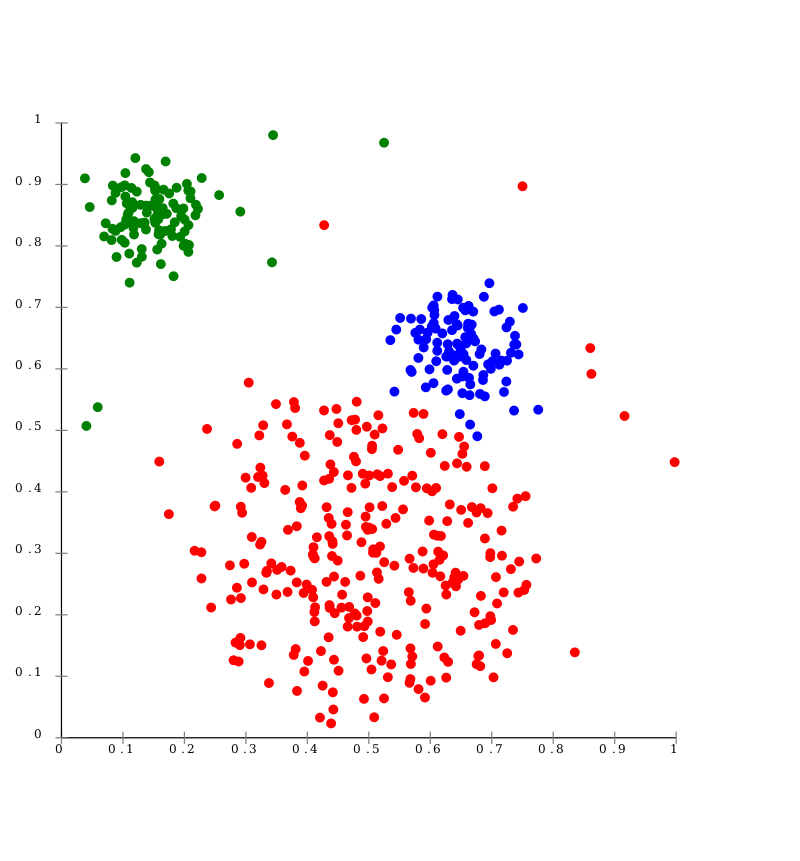
\includegraphics[scale=0.3]{ejemplo}
	\caption{Ejemplo de \textit{clustering}. \cite{chire_deutsch:_2011}}
	\label{fig:ejemplo1}
\end{figure}

El análisis clúster se aplica en numerosos campos como las ciencias naturales, médicas, económicas, \textit{marketing}, \dots En \textit{marketing}, por ejemplo, es útil dividir a los clientes y conocer las necesidades de cada segmento de mercado para lograr alcanzar a los clientes potenciales. En psicología puede ser útil encontrar tipos de personalidad a partir de los cuestionarios realizados. En arqueología se puede aplicar esta técnica para clasificar objetos en diferentes periodos.

Para llevar a cabo un análisis clúster hay que realizar principalmente dos pasos:

\begin{enumerate}
\item Elegir una medida de similitud. Dependerá del objeto de estudio, tipo de medidas (nominales, ordinales, intervalos) y tipo de variables (continuas o discretas). Lo veremos en la Sección \ref{sec:medidas}.
\item Elegir un algoritmo para construir los grupos. Hay dos grupos principales: de particionamiento y jerárquicos (que a su vez se dividen entre divisivos y aglomerativos). En la Sección \ref{sec:algoritmos} explicaremos la diferencia entre ambos grupos y veremos algunos ejemplos.
\end{enumerate}

Además, en la Sección \ref{sec:num} trataremos el problema de decidir el número de clústeres y veremos algunos métodos utilizados para determinarlo. Por último, hemos implementado un ejemplo de agrupamiento tomando los datos de las flores de iris de Fisher, el análisis se encuentra en la Sección \ref{sec:practica}.

\section{Medidas de similitud}\label{sec:medidas}

La mayoría de los esfuerzos para producir una estructura de grupo más simple a partir de un conjunto complejo de datos requiere una medida de ``cercanía'' o  ``similitud''. Habitualmente la subjetividad juega un papel importante en la elección de una medida de similitud, Algunas consideraciones importantes incluyen la naturaleza de las variables (discreta, continua, binaria), las escalas de las medidas (nominal, ordinal, intervalo) y conocimiento específico sobre el problema. En cualquier caso, los valores de las variables consideradas serán normalizados, para evitar que unas variables tengan más peso que otras a la hora de realizar el agrupamiento.

Cuando los ítems (unidades o casos) son agrupados, la proximidad se suele indicar mediante alguna medida de la distancia. En contraste, las variables se suelen agrupar según los coeficientes de correlación o medidas de asociación.

\subsection{Distancias y coeficientes de similitud para parejas de ítems}

Recordamos que la distancia euclídea entre dos observaciones $p$-dimensionales (ítems) $x' = [x_1,x_2,...,x_p]$ e $y'=[y_1,y_2,...,y_p]$ es

\[d(x,y) = \sqrt{(x_1-y_1)^2+(x_2-y_2)^2+...+(x_p-y_p)^2}=\sqrt{(x-y)^T(x-y)}.\]

La distancia estadística entre las mismas dos observaciones es de la forma:

$$d(x,y)=\sqrt{(x-y)^TA(x-y)}. $$

Normalmente, $A=S^{-1}$, donde $S$ contiene las varianzas y covarianzas de la muestra. Sin embargo, sin conocimiento previo de los distintos grupos, estas cantidades de las muestras no puede ser calculadas. Por esta razón, usualmente se prefiere la distancia euclídea para realizar \textit{clustering}.\\

Otra medida de la distancia es la métrica de Minkowski, que viene dada por:

$$ d(x,y)=\left  [\sum_{i=1}^{p}{|x_i-y_i|^m} \right ]^{1/m}.$$

Para $m=1$, $d(x,y)$ mide la distancia Manhattan entre dos puntos en $p$ dimensiones. Para $m=2$,$d(x,y)$ se convierta en la distancia euclídea. En general, variar $m$ cambia el peso dado a diferencias mayores y menores.\\

Adicionalmente, dos medidas populares de distancia o ``disimilitud'' son las dadas por la métrica de Canberra y el coeficiente de Czekanowski. Ambas medidas están definidas únicamente para variables no negativas.\\

La métrica de Canberra se define como: \[d(x,y)=\sum_{i=1}^{p}{\frac{|x_i-y_i|}{(x_i+y_i)}}.\]\\

El coeficiente de Czekanowski es: \[d(x,y)=1-\frac{2\sum_{i=1}^{p}{min(x_i,y_i)}}{\sum_{i=1}^{p}{(x_i+y_i}}.\]

Es aconsejable que cuando sea posible se utilicen distancias ``verdaderas'' para \textit{clustering}, esto es, distancias que verifiquen las propiedades de la definición matemática de distancia:
\begin{itemize}
\item $d(P,Q)=d(Q,P)$,
\item $d(P,Q)>0\ si\ P\neq Q$,
\item $d(P,Q)=0\ si\ P=Q$,
\item $d(P,Q)\leq d(P,R)+d(R,Q)$,
\end{itemize}

siendo $P$ y $Q$ dos puntos cualquiera y $R$ un punto intermedio.\\ 

Sin embargo, la mayoría de los algoritmos de \textit{clustering} aceptarán números de distancia que no satisfagan la desigualdad triangular.\\

Cuando los ítems no puedan ser representados por medidas $p$-dimensionales significativas, las parejas de ítems se suelen comparar según la presencia o ausencia de ciertas características. Ítems similares tienen más características en común que ítems desemejantes. La presencia o ausencia de una característica se puede describir matemáticamente introduciendo una variable binaria, que toma el valor 1 si la característica está presente y el valor 0 cuando la característica está ausente. 

\begin{table}[H]
  \caption{Ejemplo \ref{ej:binarizacion}, binarización de variables.}
  \label{tab:binarizacion}
\centering
  \begin{tabular}{lrrrrr}
    \toprule
  Variables    & 1    & 2    & 3   & 4   & 5   \\
  \midrule
Ítem $i$ & 1    & 0    & 0   & 1   & 1   \\
Ítem $k$ & 1    & 1    & 0   & 1   & 0\\
\bottomrule
\end{tabular}
\end{table}

En la Tabla \ref{tab:binarizacion} vemos un ejemplo (\ej{ej:binarizacion}) en el que se utilizan 5 variables binarias para medir la distancia entre los ítem $i$ y $j$. En este caso, hay dos parejas 1-1, una pareja 0-0 y dos parejas que no coinciden.\\

Sea $x_{ij}$ la puntuación (0 ó 1) de la $j$-ésima variable binaria en el $i$-ésimo ítem y sea $x_{kj}$ la puntuación de la $j$-ésima variable binaria en el $k$-ésimo ítem, con $j=1,2,...,p$. Entonces,

$$(x_{ij}-x_{kj})^2 = \left \{ \begin{matrix} 0 & \mbox{si } x_{ij}=x_{kj}
\\ 3n+1 & \mbox{si }x_{ij}\neq x_{kj}\end{matrix}\right.   $$

y la distancia euclídea al cuadrado, $\sum_{j=1}^p{(x_{ij}-x_{kj})^2}$, proporcionan una forma de contar el número de disparidades. Una distancia grande corresponde a muchas disparidades, es decir, ítems desemejantes. En el Ejemplo \ref{ej:binarizacion}, el cuadrado de las distancia entre los ítems $i$ y $k$ sería

$$\sum_{j=1}^5{(x_{ij}-x_{kj})^2}=(1-1)^2+(0-1)^2+(0-0)^2+(1-1)^2+(1-0)^2=2.$$

Aunque la distancia usada en el Ejemplo \ref{ej:binarizacion} puede ser usada para medir la similitud, tiene la desventaja de que valora por igual las parejas 1-1 y 0-0. En algunos casos, una pareja 1-1 es una indicación mayor de similitud que una pareja 0-0. Por ejemplo, al agrupar gente, que dos personas sean capaz de leer griego antiguo es una evidencia mayor de similitud que la ausencia de dicha habilidad. Para reflejar este trato diferente entre las parejas de 1-1 y 0-0, se han sugerido diversos esquemas para definir los coeficientes de similitud.\\
Para introducir dichos esquemas, vamos a organizar las frecuencias de las parejas que coinciden y las que no para los ítems $i$ y $k$ en la forma de una tabla de contingencia:

\begin{table}[H]
  \centering
  \caption{Ejemplo \ref{ej:binarizacion}, tabla de contingencia.}
  \label{tab:contingencia}
\resizebox{7cm}{!} {
  \begin{tabular}{llrrrrr}
    \toprule
\multicolumn{2}{l}{\multirow{2}{*}{}} & \multicolumn{3}{c}{Ítem $k$} & \multicolumn{2}{c}{} \\\cmidrule{3-5}
\multicolumn{2}{l}{}                  & 1        &       & 0       & \multicolumn{2}{c}{{Total}}                        \\
\midrule
{Ítem $i$}       & 1      & $a$        &       & $b$       & \multicolumn{2}{c}{$ab$}                     \\
                              & 0      & $c$        &       & $d$       & \multicolumn{2}{c}{$c+d$}                     \\ \midrule
\multicolumn{2}{l}{Total}            & $a+c$      &       & $b+d$     & \multicolumn{2}{c}{$p=a+b+c+d$}\\
\bottomrule
\end{tabular}
}
\end{table}

En la Tabla \ref{tab:contingencia}, $a$ representa la frecuencia de parejas 1-1, $b$ es la frecuencia de parejas 1-0 y así sucesivamente. Dadas las anteriores cinco parejas, $a=2$ y $b=c=d=1$.\\

La Tabla \ref{tab:similitud} lista coeficientes de similitud comunes definidos en términos de frecuencias de la Tabla \ref{tab:contingencia}.

\begin{table}[H]
  \centering
  \caption{Coeficientes de similitud para ítems \textit{clustering}.}
  \label{tab:similitud}
\resizebox{13cm}{!} {
\begin{tabular}{ll}
\toprule               
\multicolumn{1}{l}{Coeficiente} & \multicolumn{1}{l}{Fundamento}\\
\midrule
1 $\quad\frac{a+d}{p}$                            & Las parejas 1-1 y 0-0 ponderan lo mismo.\\ \\
2 $\quad\frac{2(a+d)}{2(a+d)+b+c}$                            & Las parejas 1-1 y 0-0 ponderan el doble.                                                                                                        \\\\
3 $\quad\frac{a+d}{a+d+2(b+c)}$                             & Las parejas que no coinciden ponderan el doble.                                                                                                 \\\\
4  $\quad\frac{a}{p}$                             & No hay parejas 0-0 en el numerador.                                                                                                    \\         \\
5 $\quad\frac{a}{a+b+c}$                             & \begin{tabular}[c]{@{}l@{}}No hay parejas 0-0 en el numerador ni el denominador\\ (Las parejas 0-0 son irrelevantes).\end{tabular}              \\\\
6 $\quad\frac{2a}{2a+b+c}$                             & \begin{tabular}[c]{@{}l@{}}No hay parejas 0-0 en el numerador ni el denominador.\\ Las parejas 1-1 ponderan el doble.\end{tabular}              \\\\
7 $\quad\frac{a}{a+2(b+c)}$                             & \begin{tabular}[c]{@{}l@{}}No hay parejas 0-0 en el numerador ni el denominador.\\ Las parejas que no coinciden ponderan el doble.\end{tabular} \\\\
8 $\quad\frac{a}{b+c}$                             & \begin{tabular}[c]{@{}l@{}}Proporción de parejas que coinciden (excluyendo las 0-0) en\\  relación a las parejas que no coinciden.\end{tabular} \\\\
\bottomrule
\end{tabular}
}
\end{table}

Los coeficientes 1, 2 y 3 de la Tabla \ref{tab:similitud} están monotónicamente relacionados. Supongamos que el coeficiente 1 se calcula para dos tablas de contingencia: Tabla I y Tabla II. Entonces, si $(a_I+d_I)/p \geq (a_{II}+d_{II})/p$, tenemos que $2(a_I+d_I)/[2(a_I+d_I)+b_I+c_I] \geq 2(a_{II}+d_{II})/[2(a_{II}+d_{II})+b_{II}+c_{II}]$ y el coeficiente 3 será al menos tan grande para la Tabla I como lo es para la Tabla II. Los coeficientes 5, 6 y 7 también mantienen sus órdenes relativos.\\

La monotonicidad es importante, ya que algunos procedimientos de \textit{clustering} no se ven afectados si la definición de similitud se modifica de manera que los órdenes relativos de similitud no cambian. Los procedimientos jerárquicos de asociación simple y asociación completa que se verán en la Sección \ref{sec:algoritmos} no se ven afectados Para estos métodos, cualquier elección entre los coeficientes 1, 2 y 3 de la Tabla \ref{tab:similitud} producirá las mismas agrupaciones. Análogamente, cualquier elección entre los coefcientes 5, 6 y 7 también resultará en agrupaciones idénticas.\\ % ¿Referenciar la sección de jerárquicos?

Veamos un ejemplo (\ej{ej:coef_similitud}) de cálculo de coeficientes de similitud. Supongamos cinco individuos con las características mostradas en la Tabla \ref{tab:ej-similitud}.

\begin{table}[h]
  \centering
  \caption{Individuos y características del Ejemplo \ref{ej:coef_similitud}.}
  \label{tab:ej-similitud}
\resizebox{15cm}{!} {
  \begin{tabular}{lrrrrrr}
    \toprule
            & Altura (in) & Peso (lb) & Color de ojos & Color de pelo & Mano predominante & Género \\ \midrule
Individuo 1 & 68                       & 140                    & Verde                             & Rubio                             & Derecha                               & Femenino\\
Individuo 2 & 73 & 185 & Marrón & Moreno & Derecha & Masculino                  \\
Individuo 3 & 67 & 165 & Azul & Rubio & Derecha & Masculino                  \\
Individuo 4 & 64 & 120 & Marrón & Moreno                            & Derecha & Femenino \\
Individuo 5 & 76 & 210 & Marrón & Moreno & Izquierda & Masculino                 
\end{tabular}
}
\end{table}

Definimos seis variables binarias $X_1,X_2,X_3,X_4,X_5,X_6$ como:

$$X_1 = \left \{ \begin{matrix} 1 & \mbox{si Altura}  \geq 72 
\\ 0 & \mbox{si Altura}  < 72 \end{matrix}\right.$$

$$X_2 = \left \{ \begin{matrix} 1 & \mbox{si Peso}  \geq 150 
\\ 0 & \mbox{si Peso}  < 150 \end{matrix}\right.   $$

$$X_3 = \left \{ \begin{matrix} 1 & \mbox{si Ojos marrones} 
\\ 0 & \mbox{si otro color de ojos}\end{matrix}\right.   $$

$$X_4 = \left \{ \begin{matrix} 1 & \mbox{si Pelo rubio} 
\\ 0 & \mbox{si otro color de pelo } \end{matrix}\right.   $$

$$X_5 = \left \{ \begin{matrix} 1 & \mbox{si Diestro} 
\\ 0 & \mbox{si Zurdo } \end{matrix}\right.   $$

$$X_6 = \left \{ \begin{matrix} 1 & \mbox{si Masculino} 
\\ 0 & \mbox{si Femenino}  \end{matrix}\right.   .$$

Las puntuaciones de los individuos 1 y 2 en las $p=6$ variables binarias son las encontradas en la Tabla \ref{tab:puntuaciones}.

\begin{table}[h]
  \centering
  \caption{Puntuaciones individuos 1 y 2.}
  \label{tab:puntuaciones}
\resizebox{8cm}{!} {
  \begin{tabular}{lrrrrrr}
    \toprule
            & \multicolumn{1}{l}{$X_1$} & \multicolumn{1}{l}{$X_2$} & \multicolumn{1}{l}{$X_3$} & \multicolumn{1}{l}{$X_4$} & \multicolumn{1}{l}{$X_5$} & \multicolumn{1}{l}{$X_6$} \\ \midrule
Individuo 1 & 0                        & 0                        & 0                        & 1                        & 1                        & 1                        \\
Individuo 2 & 1                        & 1                        & 1                        & 0                        & 1                        & 0\\
\bottomrule
\end{tabular}
}
\end{table}

El número de parejas que coinciden y las que no se indican en la Tabla \ref{tab:contingencias-ej}.

\begin{table}[h]
  \centering
  \caption{Tabla de contingencias para los individuos 1 y 2 del Ejemplo \ref{ej:coef_similitud}.}
  \label{tab:contingencias-ej}
\resizebox{6.5cm}{!} {
  \begin{tabular}{lrrrrr}
    \toprule
\multicolumn{2}{l}{\multirow{2}{*}{}} & \multicolumn{2}{c}{Individuo 2} & \\\cmidrule{3-4}
\multicolumn{2}{l}{}                  & 1        &   0       & \multicolumn{2}{c}{Total}                        \\ \midrule
Individuo 1      & 1      & 1        &  2       & \multicolumn{2}{c}{3}                     \\
                              & 0      & 3        &    0       & \multicolumn{2}{c}{3}                     \\ \midrule
\multicolumn{2}{l}{Total}            & 4     & 2     & \multicolumn{2}{c}{6}\\
\bottomrule
\end{tabular}
}
\end{table}

Empleando el coeficiente de similitud 1, que pondera por igual las parejas que coinciden, calculamos

$$\frac{a+d}{p}=\frac{1+0}{6}=\frac{1}{6}. $$

Continuando con el coeficiente de similitud 1, calculamos los demás números de similitud para las parejas de individuos. Mostramos los resultados en la matriz simétrica 5 x 5 a continuación.

\begin{table}[H]
\centering
\resizebox{7.5cm}{!} {
\begin{tabular}{lllllll}
\multicolumn{2}{l}{\multirow{2}{*}{}}               & \multicolumn{5}{c}{Individuo}                  \\
\multicolumn{2}{l}{}                                & 1   & 2   & 3   & 4   & 5                      \\ \cline{3-3} \cline{7-7} 
\multirow{5}{*}{Individuo} & \multicolumn{1}{l|}{1} & 1   &     &     &     & \multicolumn{1}{l|}{}  \\
                           & \multicolumn{1}{l|}{2} & 1/6 & 1   &     &     & \multicolumn{1}{l|}{}  \\
                           & \multicolumn{1}{l|}{3} & 4/6 & 3/6 & 1   &     & \multicolumn{1}{l|}{}  \\
                           & \multicolumn{1}{l|}{4} & 4/6 & 3/6 & 2/6 & 1   & \multicolumn{1}{l|}{}  \\
                           & \multicolumn{1}{l|}{5} & 0   & 5/6 & 2/6 & 2/6 & \multicolumn{1}{l|}{1} \\ \cline{3-3} \cline{7-7} 
\end{tabular}
}
\end{table}

Basándonos en las magnitudes del coeficiente de similitud, debemos concluir que los individuos 2 y 5 son los más similares mientras que los individuos 1 y 5 son los menos similiares. Si fuéramos a dividir los individuos en dos subgrupos relativamente homogéneos basándonos en los números de similitud, formaríamos los subgrupos (1 3 4) y (2 5).\\
Notar que $X_3=0$ implica una ausencia de ojos marrones, así dos personas, una con ojos azules y otra con ojos verdes, resultarán en una pareja 0-0. Por consiguiente, puede que sea inapropiado utilizar los coeficientes de similitud 1, 2 ó 3 porque estos coeficientes ponderan lo mismo las parejas 1-1 y 0-0.\\

Hemos descrito la construcción de distancias y similitudes. Siempre se pueden construir similitudes a partir de distancias. Por ejemplo, podemos fijar

$$ s_{ik} = \frac{1}{1+d_{ik}},$$ 

donde $0<s_{ik}\leq 1$ es la similitud entre los ítems $i$ y $k$ y $d_{ik}$ es la distancia correspondiente.\\
Sin embargo, no siempre podemos construir distancias ``verdaderas'', que cumplan las propiedades para \textit{clustering}, a partir de similitudes. Sólo se pueden construir si la matriz de similitudes es definida no negativa.\\
Si la matriz de similitudes fuera definida no negativa y la máxima similitud es cada de manera que $s_{ii}=1$,

$$ d_{ik}=\sqrt{2(1-s_{ik})}$$

cumple las propiedades de una distancia.

\subsection{Medidas de similitud y asociación para parejas de variables}

Hasta el momento, hemos discutido medidas de similitud para los ítems. En algunas aplicaciones, son las variables, en lugar de los ítems, las que deben ser agrupadas. Las medidas de similitud para variables suelen tomar la forma de coeficientes de correlaciones muestrales. Además, en algunas aplicaciones de \textit{clustering}, las correlaciones negativas son reemlazadas por sus valores absolutos.\\
Cuando las variables son binarias, los datos se pueden organizar en una tabla de contingencia. Sin embargo, esta vez las variables, en lugar de los ítems, definen las categorías. Para cada par de variables hay $n$ ítems categorizados en la tabla. Con la codificación usual en 0 y 1, la tabla de contingencia es como se ve en la Tabla \ref{tab:contingencia_var}. Por ejemplo, la variable $i$ vale $1$ para $a$ ítems y la variable $k$ vale $0$ para $b$ de los $n$ ítems.\\

\begin{table}[h]
  \centering
  \caption{Tabla de contingencia para un par de variables.}
  \label{tab:contingencia_var}
\resizebox{7.5cm}{!} {
\begin{tabular}{llrrrr}
\toprule
\multicolumn{2}{l}{\multirow{2}{*}{}} & \multicolumn{2}{c}{Variable $k$} & \multicolumn{2}{c}{\multirow{2}{*}{Total}} \\\cmidrule{3-4}
\multicolumn{2}{l}{}                  & 1             & 0       & \multicolumn{2}{c}{}                        \\ \hline
\multirow{2}{*}{Variable $i$}       & 1      & $a$          & $b$       & \multicolumn{2}{c}{$a+b$}                     \\
                              & 0      & c            & $d$       & \multicolumn{2}{c}{$c+d$}                     \\ \hline
\multicolumn{2}{l}{Total}            & $a+c$          & $b+d$     & \multicolumn{2}{c}{$n=a+b+c+d$}\\
\bottomrule            
\end{tabular}
}
\end{table}

La fórmula usual del coeficiente de correlación producto-momento aplicada a las variables binarias de la tabla de contingencia nos da

$$r = \frac{ad-bc}{[(a+b)(c+d)(a+c)(b+d)]^{1/2}}.$$

Este número se puede tomar como la medida de similitud entre las dos variables.\\

El coeficiente de correlación anterior se relaciona con la estadística chi-cuadrado ($r^2=\chi^2/n$) para evaluar la independencia de dos variables categóricas. Para un $n$ fijo, una similitud (o correlación) grande es consistente con la presencia de dependencia.\\

Dada la Tabla \ref{tab:contingencia_var}, se pueden desarrollar medidas de asociacion (o similitud) exactamente análogas a las listadas en la Tabla \ref{tab:similitud}. El único cambio que se requiere es la sustitución de $n$ (el número de ítems) por $p$ (el número de variables).\\

Para resumir esta sección, notamos que hay muchas medidas de similitud entre pares de objetos. Parece que la mayoría de profesionales usan distancias o los coeficientes de la Tabla \ref{tab:similitud} para el clúster de ítems y correlaciones para el clúster de variables. Sin embargo, en ocasiones, las entradas a los algoritmos de \textit{clustering} pueden ser frecuencias simples.\\

\ej{ej:leng}: Midiendo las similitudes de 11 lenguajes. Los significados de las palabras cambian a lo largo de la historia. Sin embargo, el significado de los números 1,2,3,... representa una excepción llamativa. Así, una primera comparación de lenguajes puede estar basada en exclusiva en los números naturales. La Tabla \ref{tab:leng}  nos da los 10 primeros números en inglés, polaco, húngaro y otros ocho lenguajes europeos modernos. Solamente consideramos lenguajes que utilizan el alfabeto romano y omitimos acentos y signos de puntuación.

Una observación rápida de la escritura de los números sugiere que los cinco primeros lenguajes (inglés, noruego, danés, holandés y alemán) son muy parecidos. El español, francés e italiano se parecen todavía más. El húngaro y finés parecen no estar relacionados con los demás lenguajes. El polaco tiene algunas características de los lenguajes de los subgrupos más grandes.

%Tabla 12.2 para refencias
\begin{table}[h]
\caption{Ejemplo \ref{ej:leng}. Números en 11 lenguajes.}
\label{tab:leng}
\centering
 \makebox[\textwidth][c]{
%\resizebox{16cm}{!} {
  \begin{tabular}{lllllllllll}
    \toprule
\begin{tabular}[c]{@{}l@{}}Inglés\\ (E)\end{tabular} & \begin{tabular}[c]{@{}l@{}}Noruego\\ (N)\end{tabular} & \begin{tabular}[c]{@{}l@{}}Danés\\ (Da)\end{tabular} & \begin{tabular}[c]{@{}l@{}}Holandés\\ (Du)\end{tabular} & \begin{tabular}[c]{@{}l@{}}Alemán\\ (G)\end{tabular} & \begin{tabular}[c]{@{}l@{}}Francés\\ (Fr)\end{tabular} & \begin{tabular}[c]{@{}l@{}}Español\\ (Sp)\end{tabular} & \begin{tabular}[c]{@{}l@{}}Italiano\\ (I)\end{tabular} & \begin{tabular}[c]{@{}l@{}}Polaco\\ (P)\end{tabular} & \begin{tabular}[c]{@{}l@{}}Húngaro\\ (H)\end{tabular} & \begin{tabular}[c]{@{}l@{}}Finés\\ (Fi)\end{tabular} \\ \midrule
one                                                  & en                                                    & en                                                   & een                                                     & eins                                                 & un                                                     & uno                                                    & uno                                                    & jeden                                                & egy                                                   & yksi                                                 \\
two                                                  & to                                                    & to                                                   & twee                                                    & zwei                                                 & deux                                                   & dos                                                    & due                                                    & dwa                                                  & ketto                                                 & kaksi                                                \\
three                                                & tre                                                   & tre                                                  & drie                                                    & drei                                                 & trois                                                  & tres                                                   & tre                                                    & trzy                                                 & harom                                                 & kolme                                                \\
four                                                 & fire                                                  & fire                                                 & vier                                                    & vier                                                 & quatre                                                 & cuatro                                                 & quattro                                                & cztery                                               & negy                                                  & nelja                                                \\
five                                                 & fem                                                   & fem                                                  & vijf                                                    & funf                                                 & cinq                                                   & cinco                                                  & cinque                                                 & piec                                                 & ot                                                    & viisi                                                \\
six                                                  & seks                                                  & seks                                                 & zes                                                     & sechs                                                & six                                                    & seis                                                   & sei                                                    & szesc                                                & hat                                                   & kuusi                                                \\
seven                                                & sju                                                   & syv                                                  & zeven                                                   & sieben                                               & sept                                                   & siete                                                  & sette                                                  & siedem                                               & het                                                   & seitseman                                            \\
eight                                                & atte                                                  & otte                                                 & acht                                                    & acht                                                 & huit                                                   & ocho                                                   & otto                                                   & osiem                                                & nyolc                                                 & kahdeksan                                            \\
nine                                                 & ni                                                    & ni                                                   & negen                                                   & neun                                                 & neuf                                                   & nueve                                                  & nove                                                   & dziewiec                                             & kilenc                                                & yhdeksan                                             \\
ten                                                  & ti                                                    & ti                                                   & tien                                                    & zehn                                                 & dix                                                    & diez                                                   & dieci                                                  & dziesiec                                             & tiz                                                   & kymmenen                                             \\ \bottomrule
\end{tabular}
}
\end{table}

%Tabla 12.3 para referencias
\begin{table}[h]
\caption{Ejemplo \ref{ej:leng}. Concordancia de la primera letra para 10 números en 11 lenguajes.}
\label{tab:lengConc}
\centering
\makebox[\textwidth][c]{
\begin{tabular}{lrrrrrrrrrrr}
\\
\toprule
       & E      & N      & Da     & Du     & G     & Fr    & Sp    & I     & P     & H     & Fi    \\ \midrule
E      & 10     &        &        &        &       &       &       &       &       &       &       \\
N      & 8      & 10     &        &        &       &       &       &       &       &       &       \\
Da     & 8      & 9      & 10     &        &       &       &       &       &       &       &       \\
Du     & 3      & 5      & 4      & 10     &       &       &       &       &       &       &       \\
G      & 4      & 6      & 5      & 5      & 10    &       &       &       &       &       &       \\
Fr     & 4      & 4      & 4      & 1      & 3     & 10    &       &       &       &       &       \\
Sp     & 4      & 4      & 5      & 1      & 3     & 8     & 10    &       &       &       &       \\
I      & 4      & 4      & 5      & 1      & 3     & 9     & 9     & 10    &       &       &       \\
P      & 3      & 3      & 4      & 0      & 2     & 5     & 7     & 6     & 10    &       &       \\
H      & 1      & 2      & 2      & 2      & 1     & 0     & 0     & 0     & 0     & 10    &       \\
Fi     & 1      & 1      & 1      & 1      & 1     & 1     & 1     & 1     & 1     & 2     & 10    \\ \bottomrule
\end{tabular}
}
\end{table}

Por porpósitos ilustrativos, comparamos los lenguajes mirando la primera letra de cada número. Las palabras para el mismo número son concordantes si tienen la misma primera letra y discordantes en caso contrario. De esta forma de la Tabla \ref{tab:leng} obtenemos la Tabla \ref{tab:lengConc}. Podemos observar que el inglés y el noruego comparten la misma primera letra para 8 de las 10 parejas de números. El resto de frecuencias se ha calculado de la misma forma.\\
Los resultados en la Tabla \ref{tab:lengConc} confirman la impresión visual inicial de la Tabla \ref{tab:leng}. Esto es, que el inglés, noruego, danés, holandés y alemán parecen formar un grupo. El francés, español, italiano y polaco forman otro, mientras que el húngaro y el finés no forman parte de ninguno.\\

En los ejemplo hasta el momento, hemos utilizado nuestra impresión visual de las medidas de similitud o distancia para formar grupos. En la Sección \ref{sec:algoritmos} discutiremos formas menos subjetivas para crear los clústeres, distintos algoritmos para crear los grupos. 

\section{Métodos de agrupamiento}\label{sec:algoritmos}
Un método de agrupamiento es un procedimiento de agrupación de una serie de vectores de acuerdo con un criterio. Estos criterios pueden ser, por ejemplo, la distancia o la similitud de una característica. La cercanía se define en términos de una determinada función de distancia como las vista en la Sección \ref{sec:medidas}. Aunque la medida más utilizada para calcular la simulitud entre los casos es la matriz de correlación entre los casos, también existen muchos algoritmos que se basan en la maximización de la verosimilitud.

Los métodos de agrupamiento se pueden dividir en dos tipos: jerárquicos y no jerárquicos (o de particionamiento). La principal diferencia entre ambos métodos es que en los jerárquicos una vez que se asigna un elemento a un grupo, no se puede cambiar, mientras que en los no jerárquicos sí. Además, en los métodos no jerárquicos se necesita que el número de clústers esté fijado a priori, en cambio en el agrupamiento jerárquico el propio método va fijando el número de clústers. En la Figura \ref{fig:ejemplo_metodos} observamos a la izquierda la representación de un método jerárquico (las líneas horizontales indican diferentes divisiones) y a la derecha la representación del resultado de un método de particionamiento, donde cada grupo está indicado en un color diferente).

\begin{figure}[H]
	\centering
	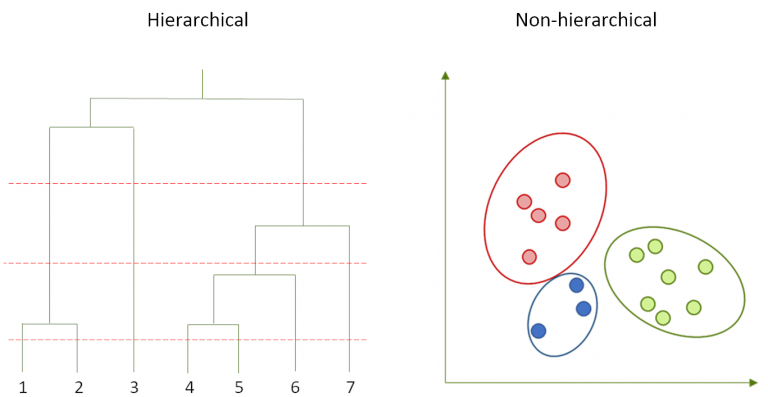
\includegraphics[scale=0.55]{victoria/compJerarquicoNoJerarquico}
	\caption{Comparación métodos jerárquico y no jerárquico.}
	\label{fig:ejemplo_metodos}
\end{figure}


\subsection{Jerárquicos}
El agrupamiento jerárquico es un método de análisis de grupos puntuales, que se basa en buscar una construcción de una jerarquía de grupos. Por tanto, los algoritmos jerárquicos van minimizando las distancias  o, visto de otra forma, maximizando  las similitudes. Es destacable que en este tipo de métodos no es necesario imponer a priori el número de grupos a formar, ya que devolverán una jerarquía de clústeres en la que según el nivel en el que nos quedemos tendremos un número u otro de grupos.

Podemos diferenciar dos técnicas para el agrupamiento jerárquico: aglomerativas y divisivas. La diferencia es que las primeras son de un acercamiento ascendente, mientras que las segundas son de un acercamiento descendente. En la Figura \ref{fig:agl_div} se simbolizan ambas técnicas.

\vspace{5mm}

\begin{figure}[H]
	\centering
	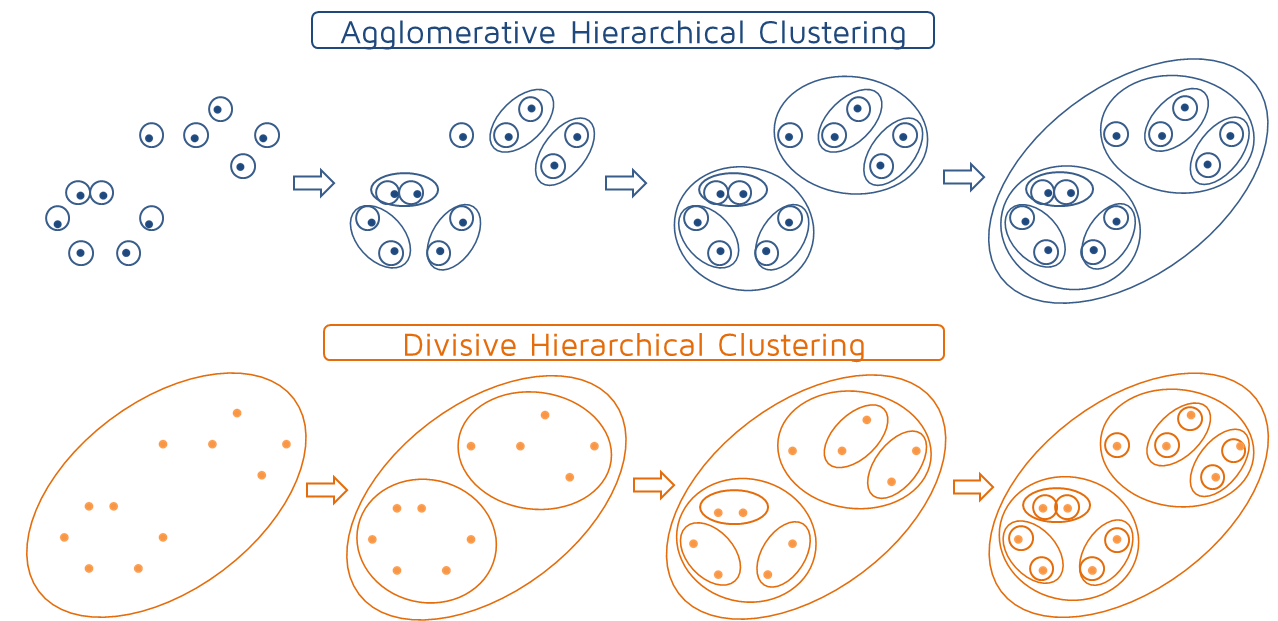
\includegraphics[scale=0.25]{victoria/compAglomeDivisivo}
	\caption{Comparación métodos aglomerativos y divisivos.}
	\label{fig:agl_div}
\end{figure}

\subsubsection{Técnicas aglomerativas}
Los algoritmos aglomerativos son prácticamente los más usados. Consisten en formar grupos o aglomerados según su similitud, uniendo los clúster que se encuentran a una menor distancia, habrá tantos clústeres al inicio como individuos haya. Estos algoritmos siguen los pasos que se muestran a continuación:

\begin{enumerate}
	\item Construir la mejor partición.
	\item Calcular la matriz distancia $D$.
	\item Repetir los siguientes pasos hasta que todos los clústeres están aglomerados. % en $\mathcal{X}$. ...no se ha definido!
	\item Encontrar los dos grupos con la distancia más cercana.
	\item Unir los dos grupos.
	\item Calcular la distancia entre los nuevos grupos y obtener una matriz de distancia reducida $D$.
\end{enumerate}

Sean $P$ y $Q$ dos grupos que vamos a unir, generando un nuevo grupo $P$ + $Q$. Ahora calculamos la distancia entre $P$ + $Q$ y $R$ utilizando la siguiente función (\ref{eq:distAglo}):

\begin{equation}\label{eq:distAglo}
	d(R, P+Q) = \delta_1 d(R,P) + \delta_2 d(R,Q) + \delta_3 d(P,Q) + \delta_4 \textvertline d(R,P) - d(R,Q) \textvertline
\end{equation}

Donde los $\delta_i$ son los factores de ponderación que dan lugar a los diferentes algoritmos de aglomeración, algunos se describen en la Tabla \ref{tab:groupDist}. Definimos $n_P$ como el número de elementos que hay en el grupo $P$, de la misma forma se definen $n_Q$ y $n_R$.

%Tabla 13.2 Härdle-Simar 2015 chapter cluster analysis
\begin{table}[H]
  \caption{Distancias entre grupos.}
  \label{tab:groupDist}
\centering
  \begin{tabular}{lrrrr}
  \toprule
  Métodos & $\delta_1$ & $\delta_2$ & $\delta_3$ & $\delta_4$  \\
  \midrule
	Single linkage & 1/2 & 1/2 & 0 & -1/2\\
	Complete linkage & 1/2 & 1/2 & 0 & 1/2\\
	Average linkage (unweighted) & 1/2 & 1/2 & 0 & 0\\
	Average linkage (weighted) & $\frac{n_P}{n_P + n_Q}$ & $\frac{n_Q}{n_P + n_Q}$ & 0 & 0\\
	Centroid & $\frac{n_P}{n_P + n_Q}$ & $\frac{n_Q}{n_P + n_Q}$ & $-\frac{n_Q n_P}{{n_P + n_Q}^2}$ & 0\\
	Median & 1/2 & 1/2 & -1/4 & 0\\
	Ward & $\frac{n_R + n_P}{n_R + n_P + n_Q}$ & $\frac{n_R + n_Q}{n_R + n_P + n_Q}$ & $-\frac{n_R}{n_R + n_P + n_Q}$ & 0\\
  \bottomrule
\end{tabular}
\end{table}

La secuencia de clúster se representan gráficamente mediante un dendrograma, esto es un digrama de datos en forma de árbol que organiza los datos en subcategorías que se van dividiendo en otros, donde se ven claramente las relaciones entre los datos y los grupos.

\begin{figure}[H]
	\centering
	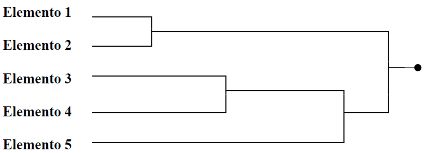
\includegraphics[scale=0.7]{victoria/aglomerativo}
	\caption{Ejemplo de dendrograma aglomerativo.}
	\label{fig:ejemplo}
\end{figure}


\subsubsection{Técnicas divisivas}
Los algoritmos divisivos parten de un único clúster y en cada iteración van dividiendo clústeres según la disimilitud entre los componentes del mismo, bajando así en la jerarquía.

En cada paso del algoritmo divisivo se deben de aplicar tres opciones:

\begin{itemize}
	\item Dividir los grupos de una forma simplificada.
	\item Dar una fórmula para evaluar cada una de las biparticiones consideradas.
	\item Dar una fórmula para determinar los niveles de nodo de la jerarquía resultante.
\end{itemize}

\begin{figure}[H]
	\centering
	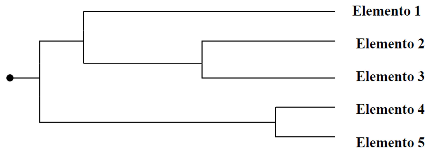
\includegraphics[scale=0.7]{victoria/disociativo}
	\caption{Ejemplo de dendrograma divisivo.}
	\label{fig:ejemplo}
\end{figure}




\subsection{No jerárquicos}
Los métodos de \textit{clustering} no jerárquicos, también denominados de particionamiento, simplemente  dividen los datos observados en un número $K$ predeterminado de grupos o clústeres, donde no hay una relación jerárquica entre la solución de $K$-clústeres y la solución de $(K+1)$-clústeres. Dado un valor $K$ buscamos una partición de los datos en $K$ clústeres de tal manera que los datos dentro de cada clúster sean similares entre ellos, mientras que los datos de diferentes clústeres están bastante diferenciados.
 
Un método de \textit{clustering} no jerárquico probablemente involucraría como primer paso la enumeración total de todos los posibles agrupamientos de los datos. Entonces, usando algún criterio de optimización, el agrupamiento que es elegido como el mejor sería la partición que optimizara dicho criterio. Claramente, para un conjunto de datos grande, tal método se vuelve rápidamente inviable, requiriendo cantidades ingentes de tiempo de procesamiento y almacenamiento. Por ello, todas las técnicas de \textit{clustering} disponibles son iterativas y trabajan con una cantidad de agrupamientos muy limitada. Los métodos no jerárquicos suelen ser computacionalmente más eficientes que los jerárquicos.

\subsubsection{$K$-Medias}

El algoritmo $K$-medias es muy popular porque es extremadamente eficiente y a menudo es usado para proyectos de \textit{clustering} de gran escala. Hacemos la observación de que el algoritmo K-medias necesita tener acceso a los datos originales.

El algoritmo $K$-medias comienza o por asignación de los datos a uno de los $K$ clústeres predeterminados y luego calculando los centroides de los $K$ \textit{$cluster$} o por pre-especificación de los centroides de los $K$ clústeres. La pre-especificación de los centroides puede ser seleccionarlos aleatoriamente o pueden ser obtenidos cortando un dendrograma a una altura apropiada. Luego, de manera iterativa, el algoritmo busca minimizar la ESS (suma de las distancias euclídeas al cuadrado, por sus siglas en inglés \textit{Euclidean Sum of Squares}) por reasignación de los datos a los clústeres. El proceso se detiene cuando no hay más reasignaciones  que reduzcan el valor de la suma.

La solución (una configuración de los datos dentro de los $K$ clústeres) puede no ser única. El algoritmo solo encontrará un mínimo local de la ESS. Es recomendable ejecutar el algoritmo varias veces usando una asignación aleatoria inicial diferente de los datos en los $K$ clústeres para encontrar el mínimo más bajo de la ESS, y por tanto, la mejor solución basada en $K$ clústeres. Los pasos del algoritmo son:
\begin{enumerate}
\item Entrada: $\textbf{L}=\{\textbf{x}_i,\ i=1,2,...,n\}$, $K$: número de clústeres.

\item Hacer uno de los siguientes:
\begin{itemize}
\item Formar una asignación aleatoria inicial de los datos en los $K$ clústeres y, para los $K$ clústeres, calcular su centroide, $\overline{\textbf{x}}_k,\ k=1,2,...,K$.
\item Pre-especificar los centroides de los K clústeres, $\overline{\textbf{x}}_k,\ k=1,2,...,K$.
\end{itemize}
\item Calcular la distancia euclídea al cuadrado para cada dato al centroide de su clúster actual:
$$ESS=\sum_{k=1}^{K}\sum_{c(i)=k}(\textbf{x}_i - \overline{\textbf{x}}_k)^T(\textbf{x}_i - \overline{\textbf{x}}_k),$$

donde $\overline{\textbf{x}}_k$ es el centroide del $k$-ésimo clúster y $c(i)$ es el clúster que contiene a $\textbf{x}_i$.

\item Reasignamos cada dato al clúster con el centroide más cercano de tal manera que ESS se reduce en magnitud. Actualizamos los centroides de los clústeres después de la reasignación de los datos. 
\item Repetimos los pasos 3 y 4 hasta que no se produzcan más reasignaciones.
\end{enumerate}

\subsubsection{Particionamiento Alrededor de Medoides (PAM)}

Este método de \textit{clustering} es una modificación del algoritmo de \textit{clustering} $K$-medoides. Aunque es similar al \textit{clustering} de $K$-medias, este algoritmo busca los $K$ ``objetos representativos'' (o medoides), en vez de los centroides, entre los datos del conjunto, y se usa una distancia basada en la disimilitud en lugar de la distancia euclídea al cuadrado. Por ello, minimiza la suma de las disimilitudes en vez de la suma de las distancias euclídeas. Este método es más robusto frente a datos anómalos como valores atípicos y valores perdidos.

Este algoritmo comienza con la matriz de proximidad $\textbf{D}=(d_{ij})$, donde $d_{ij}=d(\textbf{x}_i,\textbf{x}_j)$, ya sea dada o calculada a partir del conjunto de datos, y una configuración inicial de los datos dentro de los $K$ clústeres. Usando \textbf{D}, nosotros encontramos ese dato (llamado objeto representativo o medoide) dentro de cada clúster que minimiza la disimilitud total para todos los datos dentro de su clúster. En el algoritmo de $K$-medoides, los centroides de los pasos 2,3 y 4 en el algoritmo de $K$-medias son remplazados por los medoides, y la función objetivo ESS es sustituida por $ESS_{med}$ (definida más adelante).

El algoritmo de particionamiento alrededor de medoides (PAM) es una modificación de el algoritmo de $K$-medoides que introduce una estrategia de intercambio por la cual el medoide de cada clúster es reemplazado por otro dato de ese clúster, pero solo si este intercambio reduce el valor de la función objetivo. Una desventaja para ambos algoritmos es que aunque funciona bien en pequeños conjuntos de datos, no son suficientemente eficientes para usar en \textit{clustering} de grandes conjuntos de datos. Los pasos del algoritmo PAM son:

\begin{enumerate}
\item Entrada: $\textbf{D}=(d_{ij})$, $K$: número de clústeres.
\item Formar una asignación inicial en los K clústeres.
\item Localizar el medoide de cada clúster. El medoide del $k$-ésimo clúster esta definido como ese dato en el $k$-ésimo clúster que minimiza la disimilitud total a los otros datos dentro del clúster, $k=1,2,...,K$.


\item[$4a.$] Para el \textit{clustering} de K-medoides:
\begin{itemize}
\item Para el $k$-ésimo clúster, reasignamos el $i_k$ésimo dato al clúster con su medoide más cercano para que la función objetivo, $$ESS_{med}=\sum_{k=1}^{K}\sum_{c(i)=k}d_{ii_k}$$
sea reducida en magnitud, donde $c(i)$ es el clúster que contiene el $i$ésimo dato.
\item Repetir el paso 3 y el paso de reasignación hasta que no se produzcan mas reasignaciones.
\end{itemize}
\item[$4b.$] Para  el \textit{clustering} de particionamiento alrededor de medoides:

\begin{itemize}
\item Buscamos un dato no medoide tal que al intercambiarlo por otro medoide se produce una reducción en $ESS_{med}$, considerando el cambio que se produce en los clústeres al cambiar de medoide (si hay varios medoides que cumplen esta condición, seleccionar el que mayor reducción produzca) y se produce el cambio.

\item Repetir el proceso de intercambio hasta que no se produzca ninguna reducción del $ESS_{med}$.
\end{itemize}
\end{enumerate}

\subsubsection{Análisis difuso (fanny)}

La idea detrás del \textit{clustering} difuso es que a los datos, para ser agrupados, se les asigna probabilidades de pertenencia a cada uno de los $K$ clústeres. Sea $u_{ik}$ como denotamos a la fuerza de pertenencia del $i$-ésimo dato al $k$-ésimo clúster. Para el $i$-ésimo dato, necesitamos que $\{u_{ik}\}$ se comporte como una probabilidad. Eso es que $u_{ik}\geq0$, para todo $i$ y $k=1,2,...,K$, y $\sum_{k=1}^{K}u_{ik}=1$ para cada $i$. Esto choca con los métodos de particionamiento de $K$-medias o PAM, donde cada dato es asignado a un solo clúster.
Dada la matriz de proximidad $D=(d_{ij})$ y un número de clústeres $K$, la desconocida fuerza de pertenencia, $\{u_{ik}\}$, es encontrada minimizando la función objetivo, $$\sum_{k=1}^{K}\frac{\sum_i\sum_ju_{ik}^2u_{jk}^2d_{ij}}{2\sum_lu_{lk}^2}.$$ La función objetivo se minimiza bajo las restricciones de no negatividad y unidad de la suma usando un algoritmo iterativo.


\section{Número de clústeres}\label{sec:num}
En los algoritmos de \textit{clustering}, uno de los problemas principales es determinar el número idóneo de clústeres $ k $, el cual, es distinto al propio proceso de agrupamiento. Este procedimiento conlleva tener en cuenta varios índices. Evaluar la solución obtenida para $ k $ clústeres es similar a la práctica de determinar la dimensión del espacio en el análisis de componentes principales o el orden de los factores en análisis factorial.
La correcta elección de $ k $ suele ser ambigua ya que depende de las interpretaciones según la forma y la escala de de la distribución de los datos y la solución deseada. También hay que tener en cuenta que incluso con datos aleatorios se pueden detectar falsos clústeres. \\

En cada paso del proceso de agrupamiento se crea un nuevo clúster formado por dos observaciones, una observación y otro clúster o dos clústeres ya obtenidos. Así, el número de clústeres $ k $ decrece de $ n $ (número de observaciones) a 1. La distancia entre dos clústeres es la euclídea o la de disimilitud. %Por ejemplo, para los enlaces únicos, completos o de medias las distancias son el mínimo, máximo y la euclídea media respectivamente. Para el método de Ward, es la suma de las distancias entre clústeres al cuadrado dada en la fórmula (REFERENCIAR). 
Como $ k $ decrece de $ n $ a 1, el valor de la distancia debería aumentar ya que tendría que ser mayor cuando dos clústeres distintos se agrupan en uno solo. \\

Uno de los procedimientos para determinar el número de clústeres, por ejemplo en el algoritmo $ k$-medias, es el denominado ``método del codo'' o \textit{elbow method}. Suele ser ambiguo y no muy fiable por lo que se recomienda el uso de otras técnicas. Consiste en dibujar la gráfica de las distancia a los centros de cada clúster en función del número de clústeres. En un punto, se observará que la gráfica forma una especie de codo, de ahí nombre del método, por lo que se escoge dicho punto. Así, llamamos:\\
\[
SSE_k = \sum_{i = 1}^{n_k} = \norm{\yy_i - \bar{\yy}_k}^2,
\]
donde $ \bar{\yy}_k $ representa el centroide del clúster $ C_k $. Para cada número de clústeres $ k $ calculamos 
\[
D_k = \sum_{i = 1} ^ {k} SSE_k,
\]
y lo dibujamos en una gráfica. Si usamos el ejemplo A aportado en \cite{elbowGraph}, la gráfica sería la encontrada en la Figura \ref{fig:elbow}.

\begin{figure}[h]
	\centering
	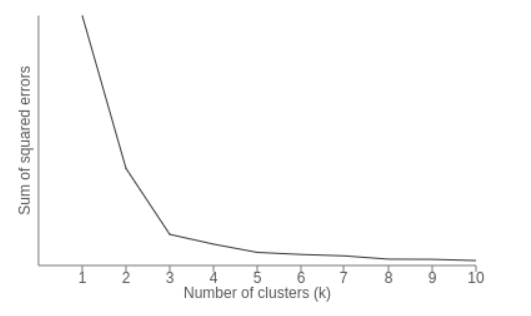
\includegraphics[scale=0.6]{pedro/elbowGraph}
	\caption{Ejemplo del método del codo.}
	\label{fig:elbow}
\end{figure}

Vemos que el cambio de de inclinación se produce cuando $ k=3 $ por lo que ese sería el número idóneo de clústeres. Hemos construido por tanto una especie de índice de separación o test de modo que si lo dibujamos en función del número de clústeres nos ayuda a identificar visualmente el $ k $ adecuado. \\

Podemos construir otra serie de índices más complejos siguiendo la misma filosofía que la anterior: construir el índice de separación o una estadística de prueba y dibujarlo en una gráfica según $ k $ de tal modo que un cambio significativo en el índice nos dé una aproximación del número de clústeres adecuado. Por ejemplo, en análisis de regresión, el coeficiente de determinación, $ R^2 $, es una medida de la varianza total de la variables dependientes según las independientes. En \textit{clustering} debemos construir un índice de $ R^2 $ que varíe en base al número de clústeres. Para $ n $ clústeres la suma total de las distancias al cuadrado es $ T = \sum_{i = 1}^{n} \norm{\yy_i - \bar{\yy}}^2 $. Así, para $ k $ clústeres definimos $ R^2 $ como
\[
R^{2}_{k} = \frac{T - \sum_k SSE_k}{T}.
\]
Para $ n $ clústeres $ SSE_k = 0 $ por lo que $ R^2 = 1 $. A medida que vamos realizando los agrupamientos, estos estarán más separados. Una gran disminución en $ R^2_k $ representaría un agrupamiento diferente. También podríamos tener en cuenta el cambio en $ R^2 $ al unir los clústeres $ R $ y $ S $ como $ SR^2 = R_k^2 - R^2_{k-1} $. El estadístico $ SR^2 $ representa, en función de $ T $, la proporción de $ SSE_t - (SSE_r + SSE_s) $ donde los clústeres $ C_R $ y $ C_S $ se han unido para formar el clúster $ C_T $.  Cuanto mayor sea el índice mayor será la pérdida de homogeneidad.\\

El objetivo del análisis clúster es encontrar el menor número de clústeres homogéneos. Para un solo clúster, la varianza agrupada para todas las variables es la media de las varianzas de cada una de las variables, es decir, $ s^2 = \sum_{i=1}^{n} \norm{\yy_i - \bar{\yy}}^2/ p(n-1)$. También podemos calcularla para un clúster $ C_k $ con $ n_k $ observaciones de la siguiente manera:
\[
s^2 = \sum_{i=1}^{n_k} \norm{\yy_i - \bar{\yy}_k}^2/ p(n_k-1).
\]
Valores grandes de la varianza agrupada indica que los clústeres no son homogéneos. Por lo tanto, si tiende a cero para algún $  k < n $ indica la formación de un clúster homogéneo. \\

Bajo una normal multivariante e independencia de los $ n $ vectores de dimensión $ p $ para $ \Sigma = \sigma^2 \textbf{I} $, podríamos hacer una prueba para verificar que los $ k $ clústeres muestran una separación significativa usando, por ejemplo, un análisis de la varianza (ANOVA) mediante una prueba $ F $ de Fisher. También podemos comprobar si dos medias están lo suficientemente separadas en cualquier nivel usando un estadístico $ t $, que son los más comunes en las pruebas $ t $ de Student. Como no es común que la independencia y la distribución normal multivariante se den a la vez, los estadísticos se denominan pseudo estadísticos $ F $ y  $ t^2 $. El pseudo estadístico $ F $ se define como
\[
F^*_k = \frac{(T-\sum_k SSE_k) / (k-1)}{\sum_k SSE_k / (n-k)}.
\]
Si $ F^*_k $ disminuye con $ k $, no deberíamos usarlo para estimar $ k $. Sin embargo, si $ F^*_k $ disminuye con $ k $ y alcanza máximo, el valor de $ k $ en el que alcanza dicho máximo o el inmediatamente anterior el candidato del número de clústeres. Por otro lado, el pseudo estadístico $ t^2 $ se define como
\[
\text{pseudo }t^2 = \frac{\lbrack SSE_t - (SSE_r + SSE_s)\rbrack(n_R + n_S - 2)}{SSE_r + SSE_s},
\]
para agrupar los clústeres $ C_R $ y $ C_S $ con $ n_R $ y $ n_S $ elementos respectivamente. De nuevo, uno puede construir la gráfica con los valores obtenidos y el número de clústeres. Si los valores son irregulares en cada punto de agrupamiento, no es un buen índice. Pero si la gráfica parece un palo de hockey, similar al método del codo, el valor $ k +1 $ que causa que la pendiente cambie es nuestro candidato a número de clústeres. \\

Varios estadísticos se generan por los programas que realizan el proceso de agrupamiento y son dibujados para evaluar heurísticamente el número de clústeres generados. Otras técnicas utilizadas para determinar el $ k $ óptimo son por ejemplo el el método de la silueta (\textit{silhouette method}) o el de la brecha (\textit{gap}).

En el \textit{silhouette method}, se observa la similitud de cada observación con su clúster en comparación con el resto de clústeres. El índice se encuentra entre los valores -1 y 1 donde un valor próximo a 1 significa un buen agrupamiento. Definimos el índice en este método para cada observación $ i $ como
\[
s(i) = \frac{b(i)-a(i)}{\max\{b(i), a(i)\}}, \hspace{2mm} \forall i = 1, \dots, n
\] 
donde $ a(i) $ es la media de la disimilitud entre $ i $ y el resto de puntos que pertenecen al mismo clúster, es decir,
\[
a(i) = \frac{1}{|C_i|-1}\sum_{j\in C_i, j \neq i} d(i,j),
\]
y $ b(i) $ como la menor distancia media de $ i $ a todos los puntos de los clústeres al que $ i $ no pertenece:
\[
b(i) = \min_{k \neq i} \frac{1}{|C_k|} \sum_{j \in C_k} d(i,j).
\] 
Destacamos que si $ |C_i| = 1 $ entonces $ s(i) = 0 $. Así, si muchos objetos tienen un valor alto indica que el resultado obtenido es satisfactorio por lo que se escoge el $ k $ que maximice el valor medio de $ s(i) $. Para ejemplificarlo, tomamos los resultados obtenidos en la referencia \cite{silouetteGraph} y se obtiene la Tabla \ref{tab:sil}.

\begin{table}[h!]
	\centering
	\begin{tabular}{lr} 
		\toprule
		k & Silhouette coeff. \\
		\midrule
		2 &  0.7049787496083262 \\			 
		3 & 0.5882004012129721 \\	
		4 &  0.6505186632729437 \\
		5 &  0.5745566973301872 \\
		6 & 0.43902711183132426 \\
		\bottomrule
	\end{tabular}
	\caption{Ejemplo \textit{silhouette method}.}
        \label{tab:sil}
\end{table}
Vemos que se obtienen los mejores resultados con 2 o 4 clústeres por lo que deberíamos decidir entre ambos según el resultado que queramos obtener. \\

Finalmente, el método de la brecha es parecido al método del codo y consiste en comparar la variación total dentro de un clúster para diferentes valores de $ k $ con sus valores esperados. El $ k $ elegido será aquel que maximice el valor de la brecha. Definimos el estadístico como:
\[
Gap(k) = E^*_n\{ \log(W_k)\} - \log(W_k).
\]
En la fórmula anterior $ E^*_n $ denota la media de una de muestra de tamaño $ n $ y 
\[
W_k = \sum_{R = 1}^{k}\frac{1}{2 n_R}\sum_{i j \in C_R} d(i,j).
\]
Notamos que se puede usar para cualquier método y distancia. Según \cite{tibshirani2001estimating} el número 2 en la fórmula de $ W_k $ es para que funcione correctamente. Visualmente se obtendría una gráfica como la mostrada en la Figura \ref{fig:gap}.

\begin{figure}[H]
	\centering
	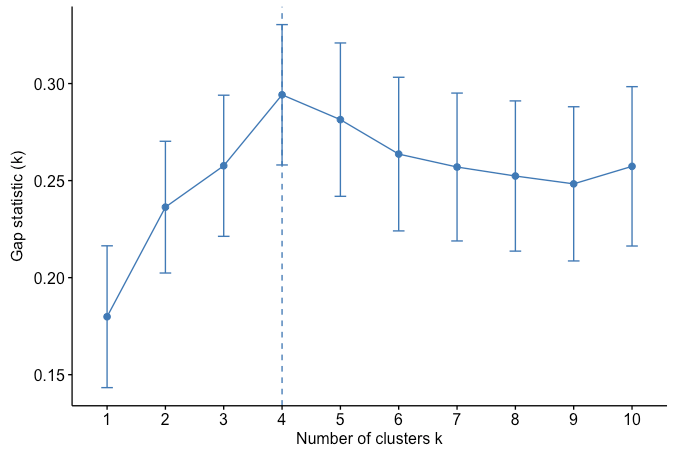
\includegraphics[scale=0.4]{pedro/gapGraph}
	\caption{Ejemplo del método de la brecha \cite{gapGraph}.}
        \label{fig:gap}
\end{figure}
Así, lo ideal sería tomar $ k = 4 $.

\section{Parte práctica}\label{sec:practica}

El objetivo de este apartado consiste en el estudio de técnicas de aprendizaje no supervisado para análisis relacional mediante segmentación. Usaremos distintos algoritmos de \textit{clustering} sobre el conjunto de datos de prueba y extraeremos conclusiones sobre los resultados obtenidos.\\

El conjunto de datos de prueba sobre el que realizaremos el estudio es el denominado conjunto de datos iris de \textbf{Fisher} \cite{noauthor_uci_nodate} que consta de un conjunto de datos multivariante introducido por \textbf{Ronald Fisher} en su artículo de 1936 (\textit{The use of multiple measurements in taxonomic problems} \cite{fisher_use_1936}) como un ejemplo de análisis discriminante lineal.\\

El conjunto de datos contiene 50 muestras de cada una de tres especies de flor \textbf{Iris} (setosa, virginica y versicolor). En él, se recogen las medidas de cuatro rasgos para cada muestra: el largo y ancho del sépalo y y el largo y ancho del pétalo, en centímetros. Basado en la combinación de estos cuatro rasgos, \textbf{Fisher} desarrolló un modelo discriminante lineal para distinguir entre una especie y otra. En las Figuras \ref{fig:setosa}, \ref{fig:virginica}, \ref{fig:versicolor} encontramos las tres especies de iris.\\

\begin{figure}[h]
  \centering
  \begin{minipage}[h]{0.29\textwidth}
    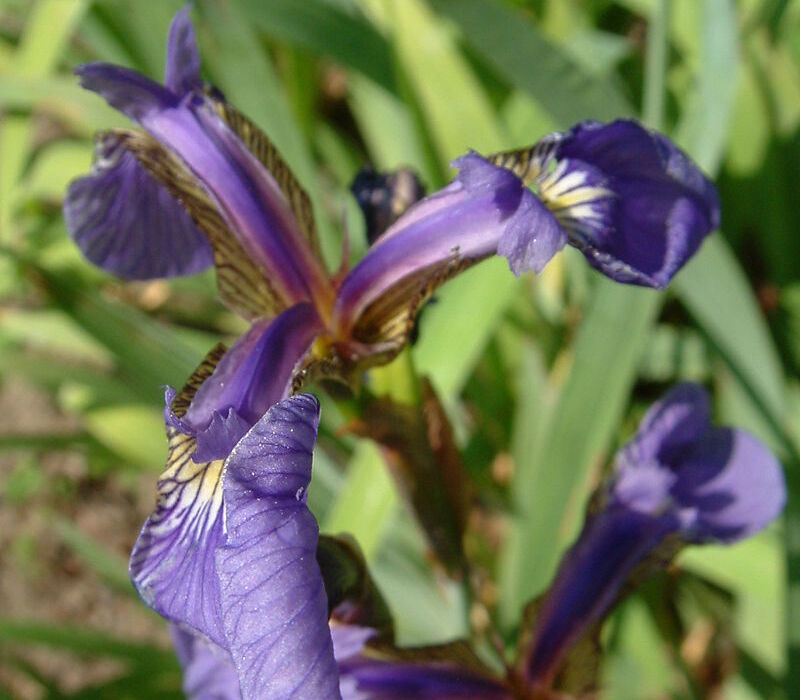
\includegraphics[width=\textwidth]{dani/setosa.jpg}
    \caption{Iris Setosa.}
  \end{minipage}
  \hfill
  \begin{minipage}[h]{0.3\textwidth}
    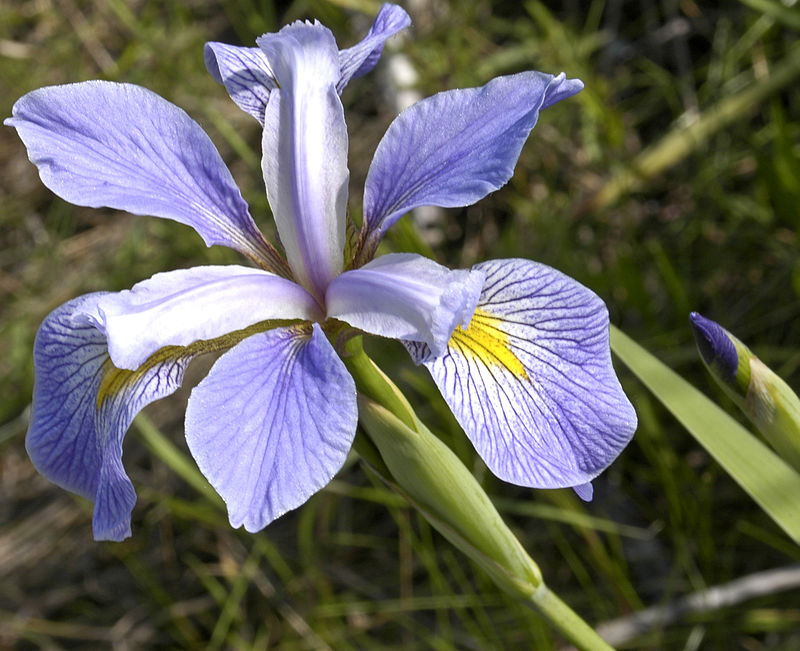
\includegraphics[width=\textwidth]{dani/virginica.jpg}
    \caption{Iris virginica.}
  \end{minipage}
  \hfill
  \begin{minipage}[h]{0.31\textwidth}
    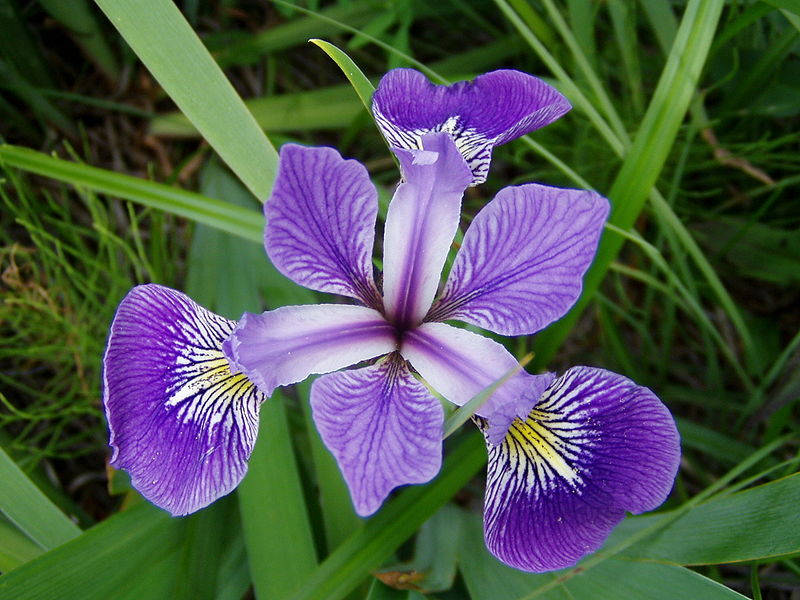
\includegraphics[width=\textwidth]{dani/versicolor.jpg}
    \caption{Iris versicolor.}
  \end{minipage}
\end{figure}

A continuación, se mostrarán los resultados obtenidos por los algoritmos en este caso de estudio. Utilizaremos una tabla comparativa donde incluiremos el nombre de los algoritmos, los resultados obtenidos por las métricas utilizadas (Calinski-Harabaz y Silhouette) y los tiempos de ejecución de los mismos. Las métricas utilizadas se interpretarán de la siguiente forma:

\begin{itemize}
\item \textbf{Calinski-Harabaz}: se basa en el concepto de densidad y de cómo de bien están separados los clústeres. Especifica la relación entre la dispersión entre distintos clústeres y la dispersión dentro de un mismo clúster. Nos indicará si estamos usando un buen número de clústeres para un algoritmo en concreto. El número óptimo de clústeres es la solución con el valor de índice Calinski-Harabasz más alto.
\item \textbf{Silhouette}: es una medida que indica cómo de similar es un objeto respecto a su propio grupo (cohesión) en comparación con otros grupos (separación). Toma valores entre -1 y +1, donde un alto valor indica que el objeto es bastante similar a su grupo y muy diferente a los de otros clúster. Si el valor es cercano a 1, la configuración de los clúster es apropiada, si no, habrá más o menos clústeres de los necesarios.
\end{itemize}

Los algoritmos elegidos han sido los siguientes: \textbf{K-Means, MeanShift, DBSCAN y Agglomerative \textit{clustering}} (\textit{clustering} jerárquico). A la hora de elegir las mejores versiones de cada algoritmo, nos basaremos en el coeficiente de Calinski-Harabaz (\textbf{CH}) que como hemos explicado antes, tendrá mayor valor si estamos usando el número adecuado de clústeres.

Mostramos en la Tabla \ref{tab:comparativa} una comparativa que contiene las mejores versiones de cada algoritmo ejecutado. Se hará un estudio más profundo sobre aquellos dos algoritmos que obtengan un mayor valor del coeficiente de Silhouette. En este caso, \textbf{K-Means} y \textbf{Agglomerative \textit{clustering}}.\\

\begin{table}[H]
\centering
\resizebox{15cm}{!} {
\begin{tabular}{lrrrrr}
\toprule
\textbf{Nombre} & \textbf{Nº clústeres} & \textbf{CH} & \textbf{SH} & \textbf{Tiempo ($s$)} & \textbf{Clústeres}                                                                                                          \\ \midrule
K-Means       & 3                    & 359.845074 & 0.504769    & 0.016456      & \begin{tabular}[c]{@{}c@{}}0:    61 (40.67\%)\\
1:    50 (33.33\%) \\2:    39 (26.00\%)\end{tabular}\\ \\
DBSCAN        & 4                   &  94.991819   & 0.306404   &  0.002353      & \begin{tabular}[c]{@{}c@{}}0:    45 (30.00\%)
\\1:    39 (26.00\%)
\\-1:    36 (24.00\%)
\\2:    30 (20.00\%)\end{tabular} \\ \\
AggCluster    & 3                    & 349.254185 & 0.504800    & 0.019058      & \begin{tabular}[c]{@{}c@{}}0:    67 (44.67\%)
\\1:    50 (33.33\%)
\\2:    33 (22.00\%)\end{tabular}                       \\ \\
MeanShift     & 3                    & 290.470683  & 0.476961    & 0.289073      & \begin{tabular}[c]{@{}c@{}}0:    81 (54.00\%)
\\1:    50 (33.33\%)
\\2:    19 (12.67\%)\end{tabular}                                             \\ \bottomrule
\end{tabular}
}
\caption{Tabla comparativa algoritmos.}
\label{tab:comparativa}
\end{table}

\clearpage

\subsection{K-Means}

K-Means es un algoritmo de clasificación no supervisada (clusterización) que agrupa objetos en K grupos basándose en sus características. El agrupamiento se realiza minimizando la suma de distancias entre cada objeto y el centroide de su grupo o clúster.\\ 

El algoritmo K-Means resuelve un problema de optimización, siendo la función a optimizar (minimizar) la suma de las distancias cuadráticas de cada objeto al centroide de su clúster. Es necesario especificar el valor de K previamente antes de ejecutar el algoritmo.\\

Para el algoritmo K-Means se ha utilizado el siguiente código en python y se ha obtenido la siguiente agrupación de las muestras:\\

\begin{lstlisting}[language=Python]
KMeans(init='k-means++', n_clusters=3, n_init=5, random_state=12345)

0:    61 (40.67%)
1:    50 (33.33%)
2:    39 (26.00%)
\end{lstlisting}\

Se mostrarán 4 gráficas realizadas y se hará un estudio sobre los resultados obtenidos. Las gráficas obtenidas para este caso, serán \textbf{Scatter Matrix, Heatmap, KPlot y BoxPlot} que mostrarán la matriz de dispersión de las muestras, mapa de calor de los centroides para cada variable y distribución de las muestras según cada variable.\\

En la Figura \ref{smkm} se representa la matriz de dispersión de las 150 muestras agrupadas en 3 clústeres: donde el clúster 0 representa las \textbf{Iris} versicolor, el clúster 1 setosa y el clúster 2 virginica. Un gráfico de matriz de dispersión es una herramienta de exploración de datos que permite buscar patrones y relaciones entre diferentes muestras en una distribución multivariante. En el gráfico se muestra el gráfico de dispersión para cada par de variables seleccionadas y una serie de histogramas en la diagonal mostrando la distribución de valores para cada una de las variables.\\

En la Figura \ref{hmkm} y \ref{kpkm} podemos ver la media y forma de las distribuciones de cada variable para cada clúster generado con el algoritmo K-Means. En el HeatMap, podemos observar la media de los centroides y podemos hacernos una idea de las características claves para clasificar cada muestra en uno de los tres tipos de flor de \textbf{Iris}.\\

Las muestras del clúster 1 (tipo setosa) se caracteriza por tener un pétalo corto y delgado, mientras que el ancho del sépalo es más ancho que la media. Las del clúster 2 (tipo virginica), se caracterizan por tener un pétalo y sépalo más grandes respecto a los otros tipos y las del clúster 3 (tipo versicolor) tienen un pétalo similar al de la virginica pero se caracteriza por tener el sépalo un poco más delgado. Podemos observar que las flores más dificiles de diferenciar serán las de los tipos virginica y versicolor puesto que tienen más características en común. Esto se puede visualizar en la matriz de dispersión y en la Figura \ref{kpkm}.

\clearpage

\begin{figure}[h]
\centering
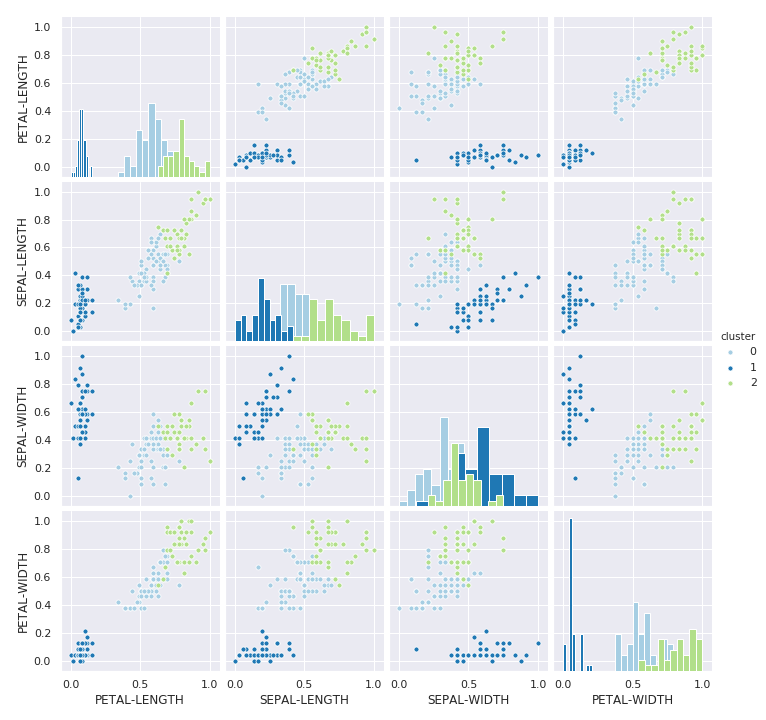
\includegraphics[scale=0.63]{dani/scatmatrixK-MeansIRIS.png}
\caption{Scatter Matrix para K-Means con 3 clústeres.}
\label{smkm}
\end{figure}\

\begin{figure}[h]
\centering
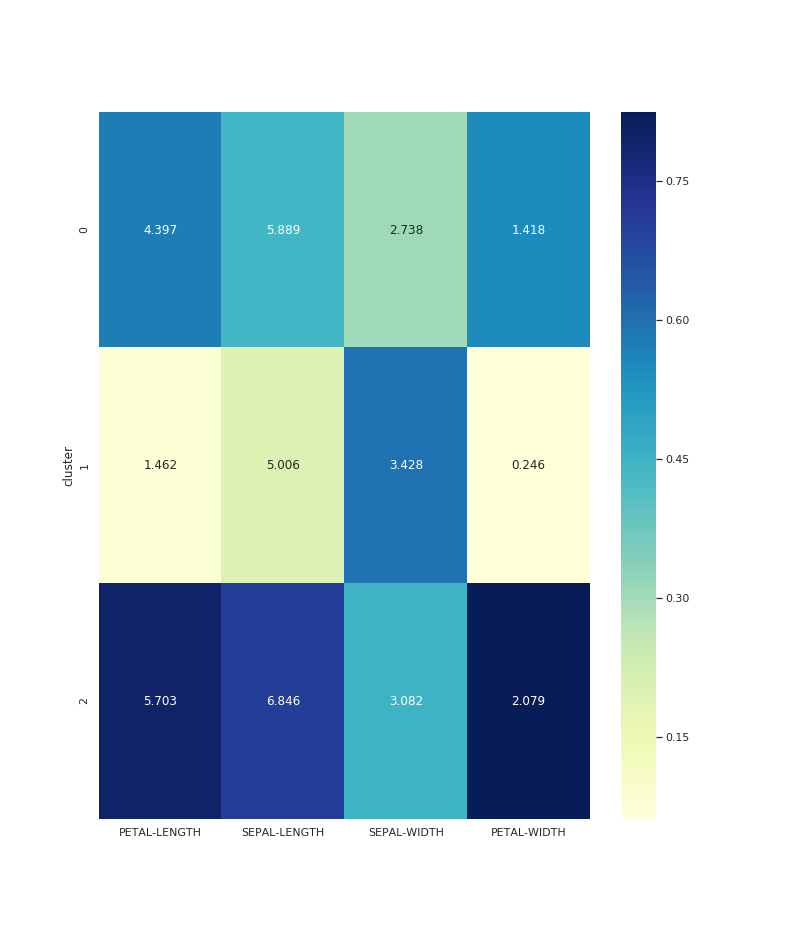
\includegraphics[scale=0.63]{dani/heatmapK-MeansIRIS.png}
\caption{HeatMap para K-Means con 3 clústeres.}
\label{hmkm}
\end{figure}


\begin{figure}[h]
\centering
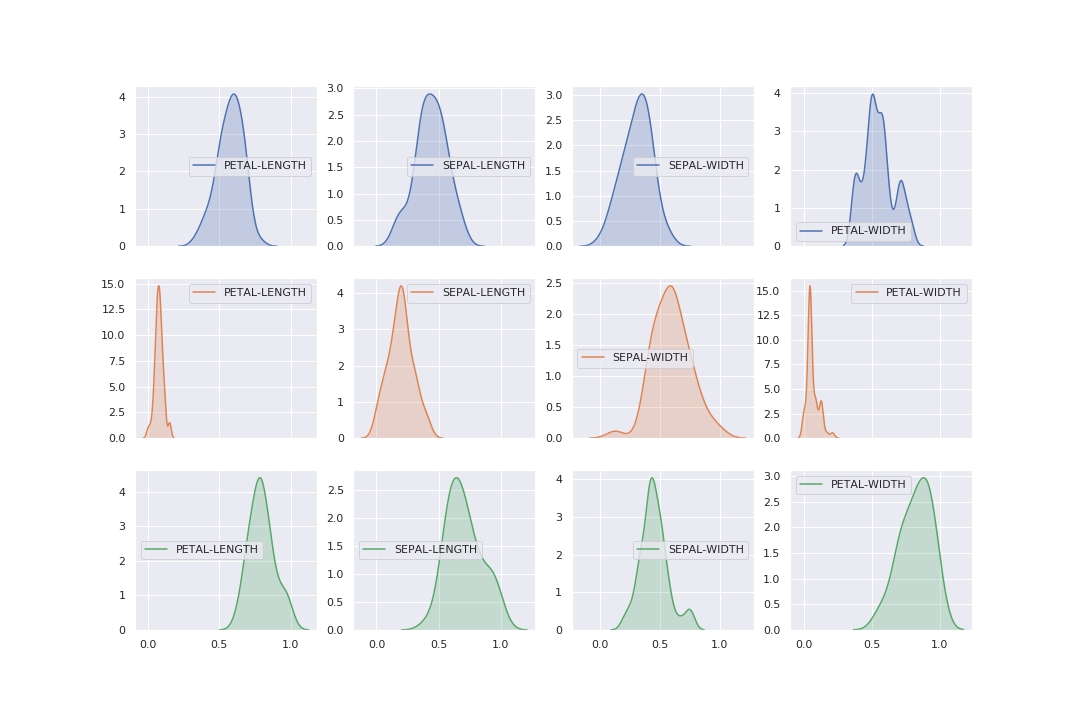
\includegraphics[scale=0.41]{dani/kdeplotK-MeansIRIS.png}
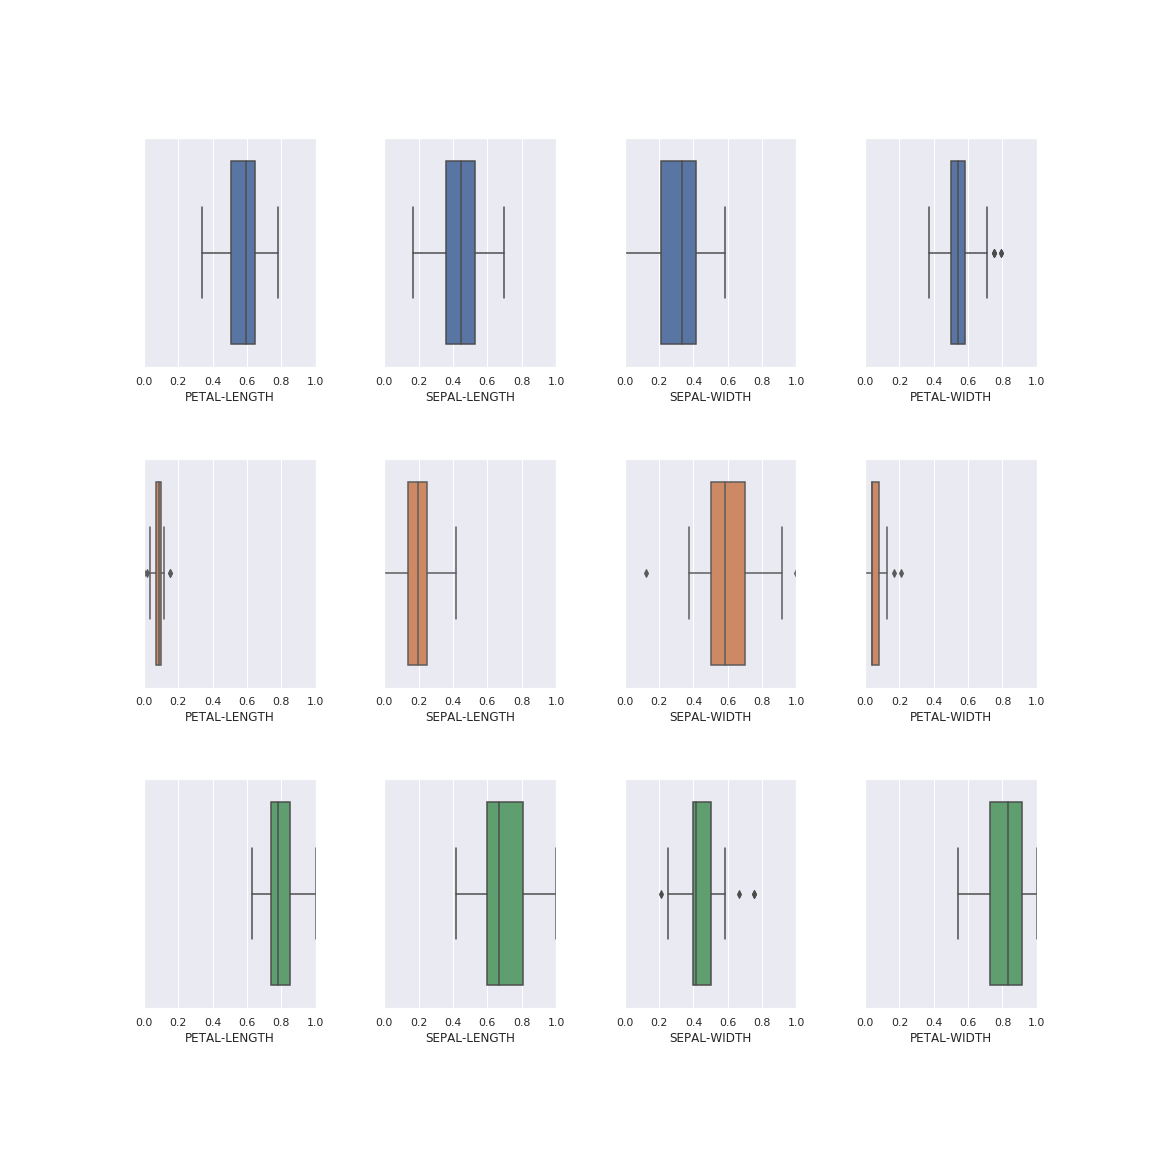
\includegraphics[scale=0.31]{dani/boxplotK-MeansIRIS.png}
\caption{KPlot y BoxPlot para K-Means con 3 clústeres.}
\label{kpkm}
\end{figure}

\clearpage

\subsection{Agrupamiento Jerárquico}

El agrupamiento jerárquico es un método de análisis de grupos puntuales, el cual busca construir una jerarquía de grupos. Estrategias para agrupamiento jerárquico generalmente caen en dos tipos: 

\begin{itemize}
\item \textbf{Aglomerativas}: Este es un acercamiento ascendente: cada observación comienza en su propio grupo, y los pares de grupos son mezclados mientras uno sube en la jerarquía.
\item \textbf{Divisivas}: Este es un acercamiento descendente: todas las observaciones comienzan en un grupo, y se realizan divisiones mientras uno baja en la jerarquía.
\end{itemize}

En general, las mezclas y divisiones son determinadas con un Algoritmo Greedy. Los resultados del agrupamiento jerárquico son usualmente presentados en un dendrograma.\\

En orden de decidir qué grupos deberían ser combinados se requiere una medida de disimilitud entre conjuntos de observaciones. En la mayoría de los métodos de agrupamiento jerárquico, esto se consigue mediante el uso de una métrica apropiada (una medida de distancia entre pares de observaciones), y un criterio de enlace el cual determina la distancia entre conjuntos de observaciones como una función de las distancias entre observaciones dos a dos.\\

En nuestro caso, usaremos la estrategia de agrupamiento aglomerativo y usaremos la métrica euclídea junto con el criterio de enlace ward (el decrecimiento en la varianza para los grupos que están siendo mezclados).\\

Para el algoritmo jerárquico aglomerativo, se ha utilizado el siguiente código en python y se ha obtenido la siguiente agrupación de las muestras:\\

\begin{lstlisting}
AgglomerativeClustering(n_clusters=3, linkage="ward", affinity='euclidean')

0:    67 (44.67%)
1:    50 (33.33%)
2:    33 (22.00%)
\end{lstlisting}\

Se mostrarán 4 gráficas realizadas y se hará un estudio sobre los resultados obtenidos. Las gráficas obtenidas para este caso, serán la matriz de dispersión y mapa de calor también usados para el método de K-Means y ademaś se mostrarán dos dendrogramas para representar el proceso de agrupamiento seguido.\\

Podemos observar que la matriz de dispersión generada por este algoritmo se asemeja mucho a la obtenida por el algoritmo K-Means. Las conclusiones que podemos extraer de las Figuras \ref{smac} y \ref{hmac} son similares a las que ya hemos comentado en el apartado anterior, por lo que nos limitaremos a extraer conclusiones sobre el dendrograma.

\clearpage

\begin{figure}[h]
\centering
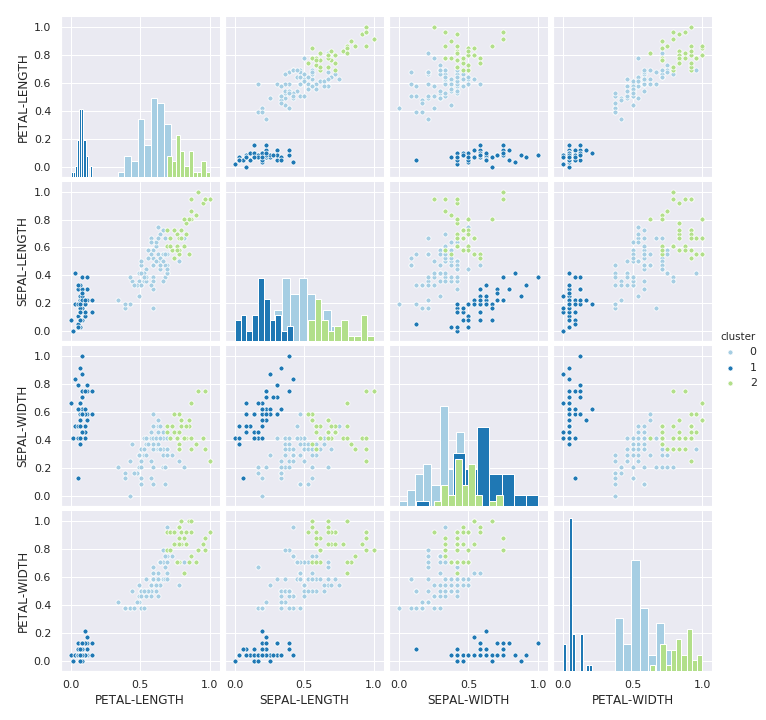
\includegraphics[scale=0.64]{dani/scatmatrixAggClusterIRIS.png}
\caption{Scatter Matrix para Agglomerative \textit{clustering} con 3 clústeres.}
\label{smac}
\end{figure}

\clearpage

\begin{figure}[h]
\centering
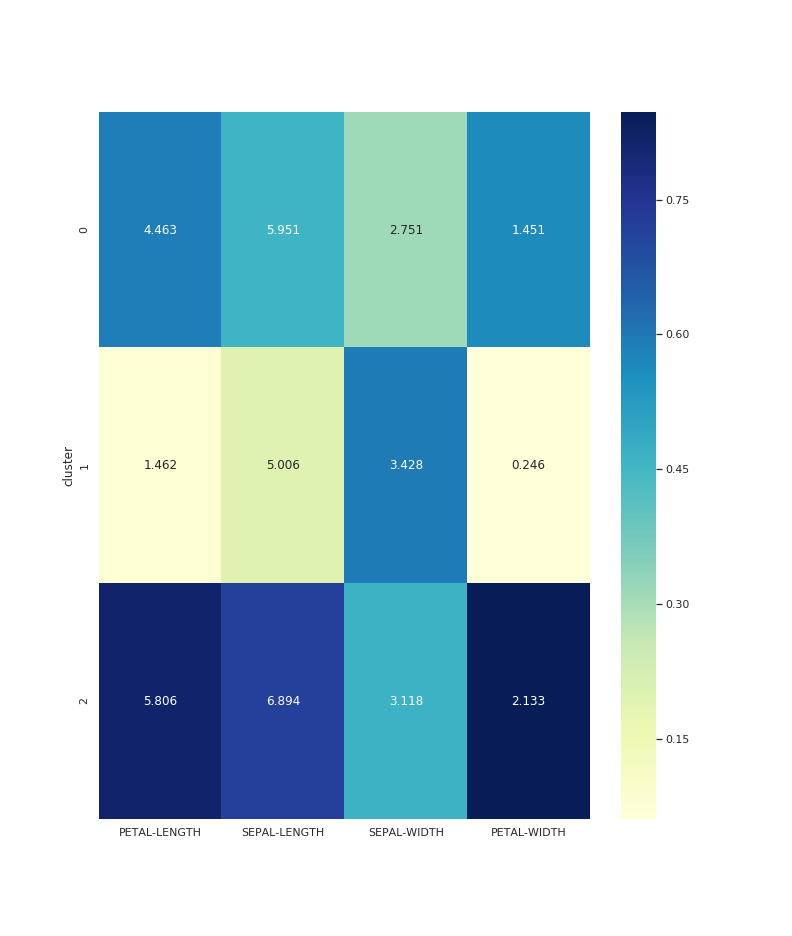
\includegraphics[scale=0.63]{dani/heatmapAggClusterIRIS.png}
\caption{HeatMap para Agglomerative \textit{clustering} con 3 clústeres.}
\label{hmac}
\end{figure}

\clearpage

\subsubsection{Dendrogramas}

Un dendrograma es un diagrama de árbol que muestra los grupos que se forman al crear clústers de observaciones en cada paso y sus niveles de similitud. En nuestro caso medimos el nivel de similitud en el eje horizontal y las diferentes muestras en el eje vertical.\\

Para ver los niveles de similitud, seleccionaremos una línea vertical del dendrograma. El patrón de cómo los valores de similitud/desimilitud cambian de un paso a otro será clave en la agrupación final para los datos.\\

La decisión acerca de la agrupación final también se conoce como cortar el dendrograma. Cortar el dendrograma es similar a trazar una línea a lo largo del dendrograma para especificar la agrupación final. También se pueden comparar diferentes agrupaciones finales en los dendrogramas para determinar cuál de ellas tiene más sentido para los datos.\\

En nuestro caso hemos impuesto que existan 3 clústers por lo que podríamos cortar el dendrograma a distancia 1, obteniendo el número elegido. Las muestras de color verde representarían a las \textbf{Iris} setosa y las de color rojo a las versicolor y virginica.

\begin{figure}[h]
\centering
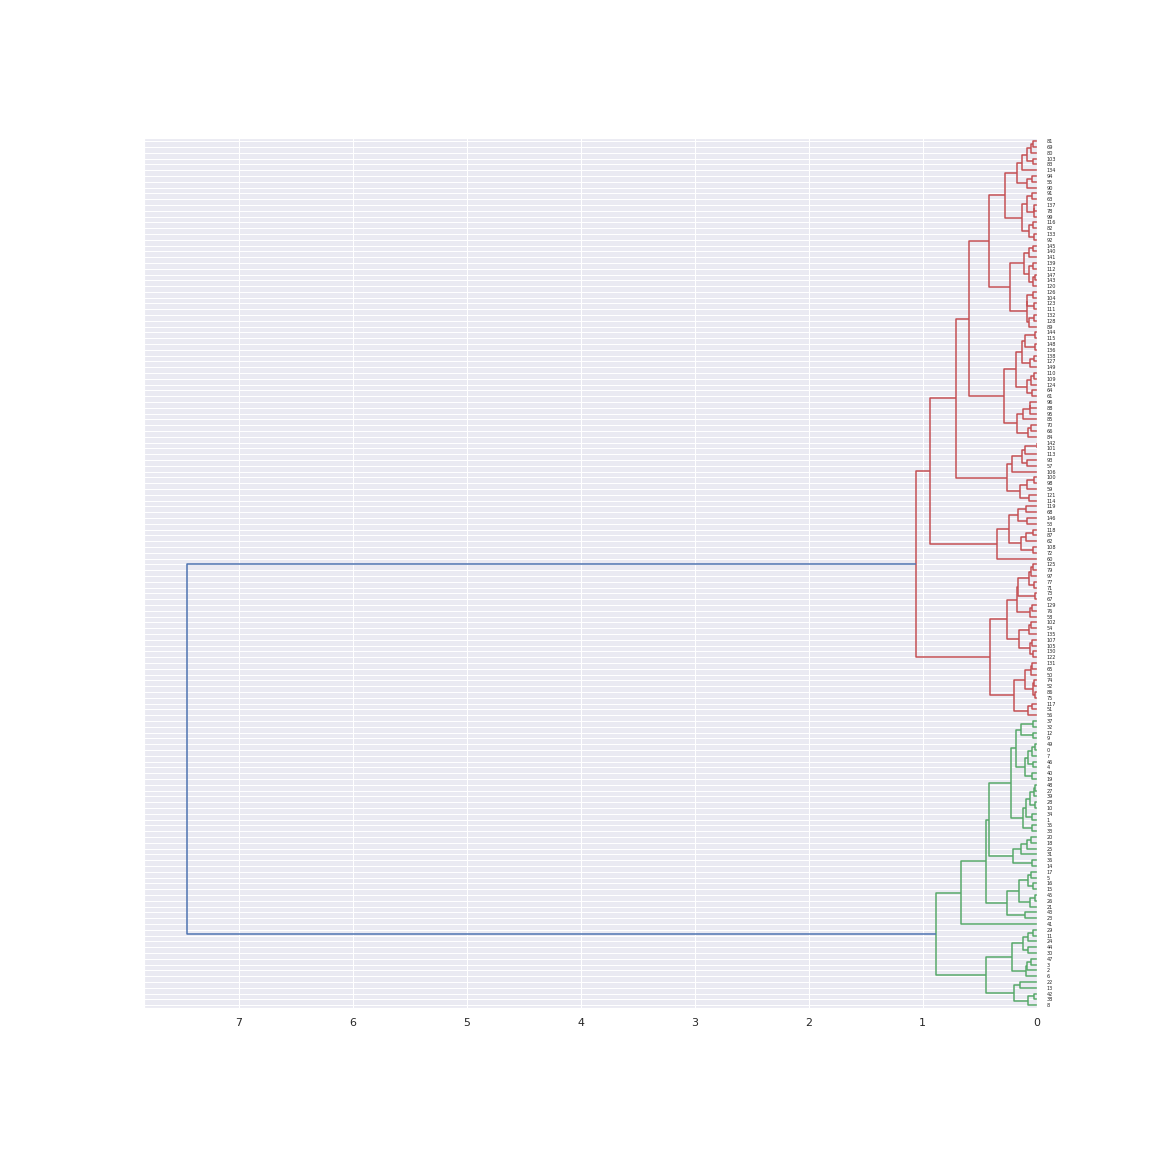
\includegraphics[scale=0.35]{dani/dendrogramAggClusterIRIS.png}
\caption{Dendrograma para Agglomerative \textit{clustering} con 3 clústeres.}
\label{dac}
\end{figure}

\clearpage

\begin{figure}[h]
\centering
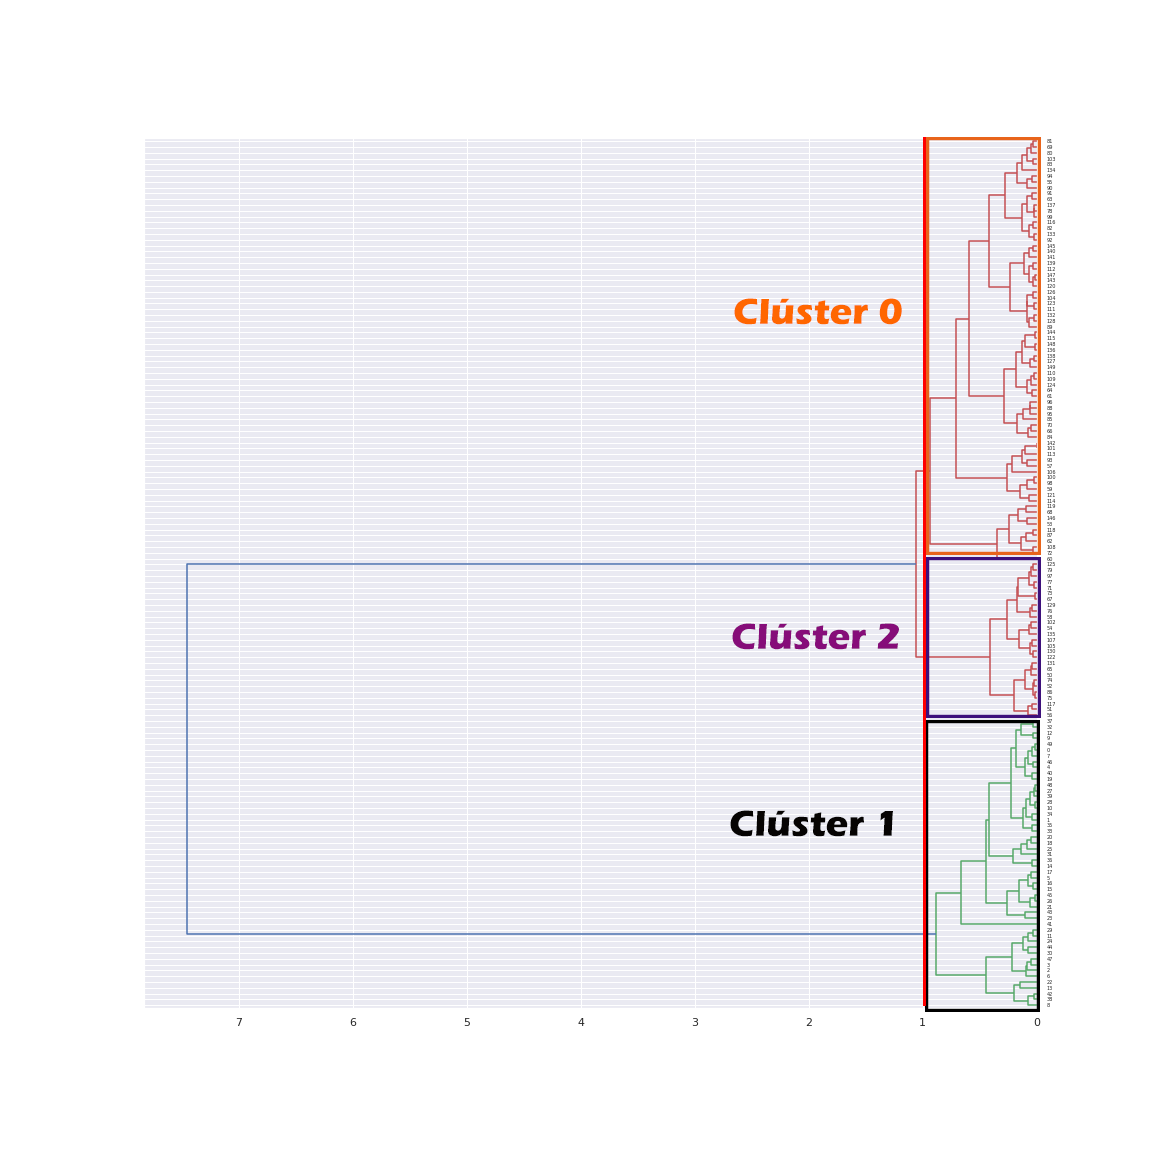
\includegraphics[scale=0.35]{dani/dendrogramcolor.png}
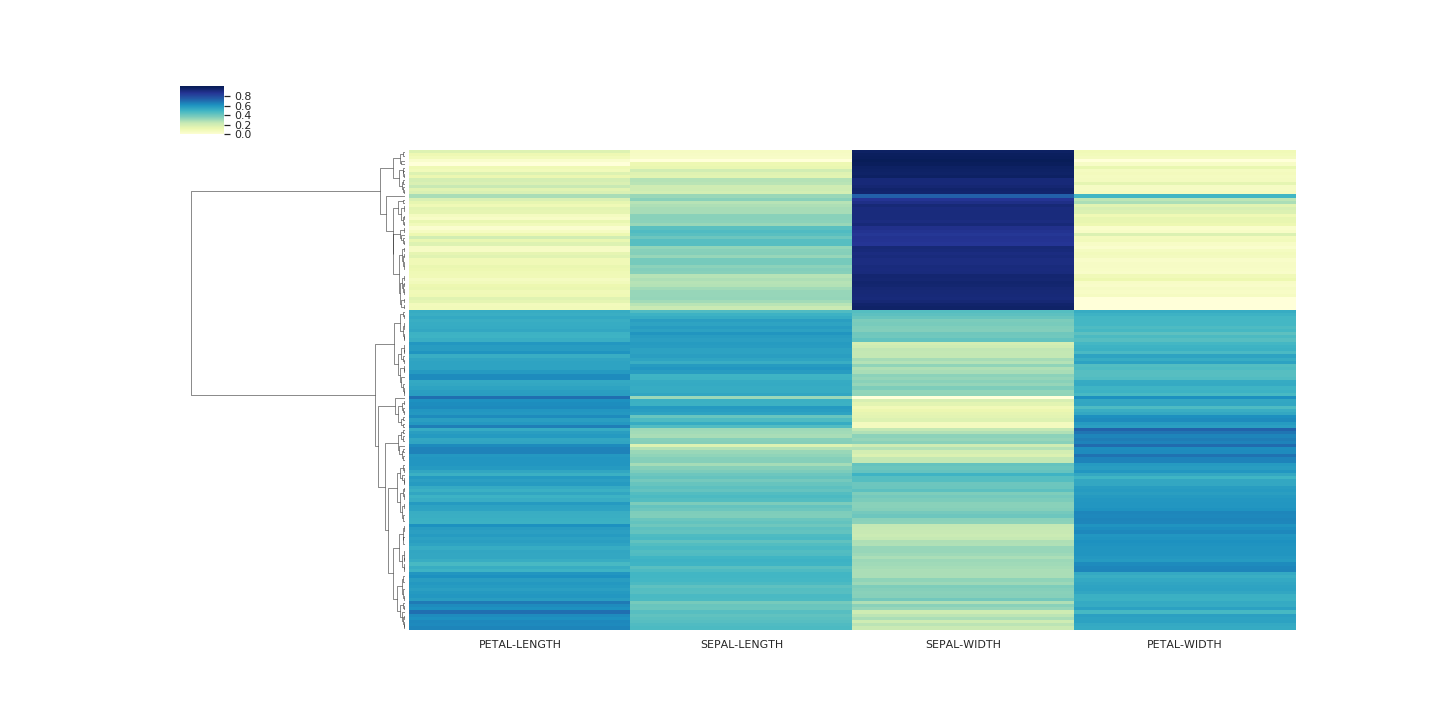
\includegraphics[scale=0.35]{dani/dendscatAggClusterIRIS.png}
\caption{Dendrogramas para Agglomerative \textit{clustering} con 3 clústeres.}
\label{dac}
\end{figure}

\clearpage

\subsection{DBSCAN}

Al contrario de la estrategia seguida por K-Means, DBSCAN (\textit{Density-Based Spatial \textit{clustering} of Applications with Noise}) no presupone clústeres convexos, sino que se basa en la densidad de las muestras para identificar los clústeres. Por este motivo, los clústeres identificados por DBSCAN pueden ser de cualquier forma.\\

Dos parámetros importantes para definir este algoritmo son: \textbf{eps}, máxima distancia entre dos muestras para poder ser consideradas pertenecientes al mismo "vecindario", y \textbf{min\_samples}, número de muestras en un vecindario para que una región pueda ser considerada densa.\\

Consideremos un conjunto de puntos a ser agrupados en un espacio determinado. La técnica de agrupación DBSCAN clasifica los puntos como puntos núcleo, puntos (densamente-)alcanzables, o ruido de la siguiente forma:

\begin{itemize}
\item Un punto $p$ pertenece al núcleo si al menos \textit{min\_samples} puntos están a una distancia $\epsilon$ de él y esos puntos son directamente alcanzables desde $p$. No es posible tener puntos directamente alcanzables desde un punto distinto al núcleo.
\item Un punto $q$ es alcanzable desde $p$ si existe una secuencia de puntos $p_1\dots p_n$ donde $p_1=p$ y $p_n=q$ y cada punto $p_{i+1}$ es directamente alcanzable desde $p_i$.
\item Un punto que no sea alcanzable desde cualquier otro se considera ruido.
\end{itemize}

Si $p$ es un punto núcleo, este forma un clúster junto a otros puntos que sean alcanzables desde él. Cada clúster contiene al menos un punto núcleo. Los puntos no núcleos alcanzables pueden pertenecer a un clúster pero actúan como una barrera puesto que no es posible alcanzar más puntos desde estos.\\

Se puede observar que la relación de ser alcanzable no es simétrica. Por definición, ningún punto puede ser alcanzable desde un punto que no sea núcleo, sin importar la distancia a la que se encuentre. Por lo tanto la noción de connectividad es necesaria para definir formalmente la extensión de un clúster dada por DBSCAN. Dos puntos $p$ y $q$ están conectados densamente si existe un punto $o$ tal que ambos $p$ y $q$ sean directamente alcanzables desde $o$. La relación estar densamente conectado es simétrica.\\

Por tanto un clúster generado por el método DBSCAN satisface dos propiedades:

\begin{itemize}
\item Todos los puntos de un mismo clúster están densamente conectados entre sí.
\item Si un punto $A$ es densamente alcanzable desde cualquier otro punto $B$ del clúster, entonces $A$ también forma parte del clúster.
\end{itemize}

Para DBSCAN, se ha utilizado el siguiente código en python y se ha obtenido la siguiente agrupación de las muestras, donde el clúster -1 representa las muestras formadas por ruido:\\

\begin{lstlisting}
DBSCAN(eps=0.12, min_samples=5)

0:    45 (30.00%)
1:    39 (26.00%)
-1:    36 (24.00%)
2:    30 (20.00%)
\end{lstlisting}\

Las gráficas obtenidas para este caso, serán la matriz de dispersión (Scatter Matrix) y mapa de calor (HeatMap).\\

En este caso podemos ver como tenemos un cuarto clúster formado por las muestras que han sido consideradas "ruido" por el algoritmo DBSCAN. Este clúster se identifica con el número -1 y contiene las muestras no alcanzables para el algoritmo con los parámetros que hemos especificado.

\begin{figure}[h]
\centering
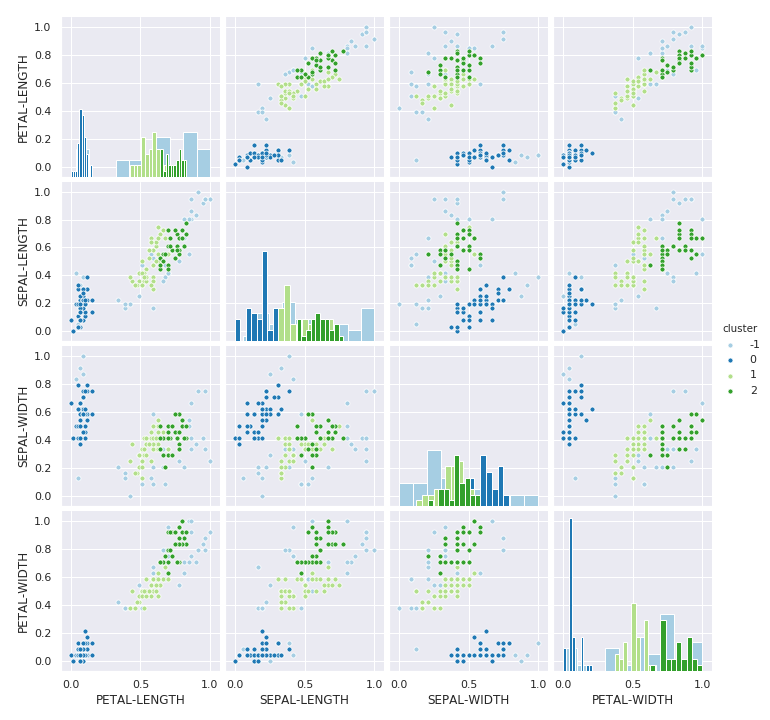
\includegraphics[scale=0.64]{dani/scatmatrixDBSCANIRIS.png}
\caption{Scatter Matrix para DBSCAN con 4 clústeres.}
\label{smdb}
\end{figure}

\clearpage

\begin{figure}[h]
\centering
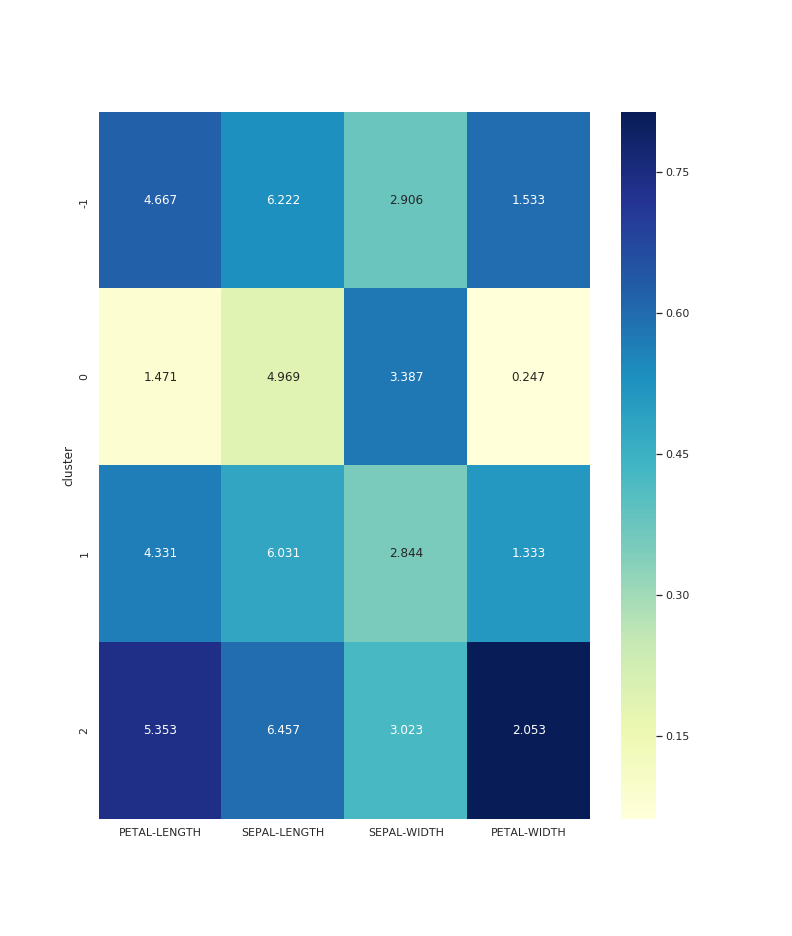
\includegraphics[scale=0.62]{dani/heatmapDBSCANIRIS.png}
\caption{HeatMap para DBSCAN con 4 clústeres.}
\label{hmdb}
\end{figure}

\clearpage

\subsection{Mean Shift}

Mean Shift es una técnica de análisis de espacio de características no paramétrica para localizar los máximos de una función de densidad. Es un método iterativo que parte de una estimación inicial $x$. Dada una función núcleo $K(x_i-x)$. Esta función determina el peso de los puntos cercanos para la reestimación de la media. Normalmente se usa un núcleo gaussiano en la distancia de la estimación actual, $K(x_i-x)=e^{-c||x_i-x||^2}$. La media ponderada de la densidad en la ventana determinada por K es:

$$m(x)=\dfrac{\sum_{x_i\in N(x)}K(x_i-x)x_i}{\sum_{x_i\in N(x)}K(x_i-x)}$$

donde $N(x)$ es el vecindario de x, un conjunto de puntos donde $K(x_i)\neq0$.\\

La diferencia $m(x)-x$ se denomina Mean Shift. El algoritmo establece $m(x)\rightarrow x$ y repite la estimación hasta que $m(x)$ converja.\\

Todavía no se conoce una prueba rígida de la convergencia del algoritmo utilizando un núcleo general en un espacio de alta dimensión. Aliyari Ghassabeh mostró la convergencia del algoritmo de cambio medio en una dimensión con una función de perfil diferenciable, convexa y estrictamente decreciente. Sin embargo, el caso unidimensional tiene aplicaciones limitadas en el mundo real.\\

Además, se ha demostrado la convergencia del algoritmo en dimensiones superiores con un número finito de los puntos estacionarios (o aislados). Sin embargo, no se han proporcionado condiciones suficientes para que una función general del núcleo tenga puntos estacionarios finitos (o aislados).\\

Sea un conjunto de datos finito $S$ embebido en el espacio euclídeo n-dimensional $X$. Sea $K$ un núcleo plano que tiene como función característica en X:

$$K(x)=\left\{
1 \ si \ ||x||\leq \lambda \atop
0 \ si \ ||x||> \lambda
\right.$$

En cada iteración del algoritmo, se establece $m(x)\rightarrow x$ para todo $s\in S$ simultáneamente. Una de las preguntas que nos podemos hacer es, cómo estimar la función de densidad dado un conjunto escaso de muestras. Uno de los enfoques más simples es simplemente suavizar los datos, por ejemplo, convolucionándolos con un núcleo fijo de ancho $h$:

$$f(x)=\sum_i K(x-x_i)=\sum_i k\dfrac{||x-x_i||^2}{h^2}$$

donde $x_i$ son las muestras de entrada y $k$ la función núcleo y h es el único parámetro que toma el algoritmo que se denomina \textit{bandwidth}. Una vez que hemos calculado $f(x)$ a partir de la ecuación anterior, podemos encontrar sus máximos locales utilizando el ascenso de gradiente o alguna otra técnica de optimización.\\

Usando esta aproximación por fuerza bruta hace que el problema sea computacionalmente inviable conforme aumentamos las dimensiones del problema sobre el espacio de búsqueda total. Por tanto, Mean Shift utiliza la técnica del reinicio de gradiente descendiente múltiple, la cual empieza desde un máximo local $y_k$ y calcula su aproximación $f(x)$ y avanza en esa dirección.

\clearpage

Para Mean Shift, se ha utilizado el siguiente código en python y se ha obtenido la siguiente agrupación de las muestras:\\

\begin{lstlisting}
MeanShift(bandwidth=estimate_bandwidth(X_normal, quantile=0.67, 
	  n_samples=400), bin_seeding=True)

0:    81 (54.00%)
1:    50 (33.33%)
2:    19 (12.67%)
\end{lstlisting}\

Las gráficas obtenidas para este caso, serán la matriz de dispersión (Scatter Matrix) y mapa de calor (HeatMap).\\

\begin{figure}[h]
\centering
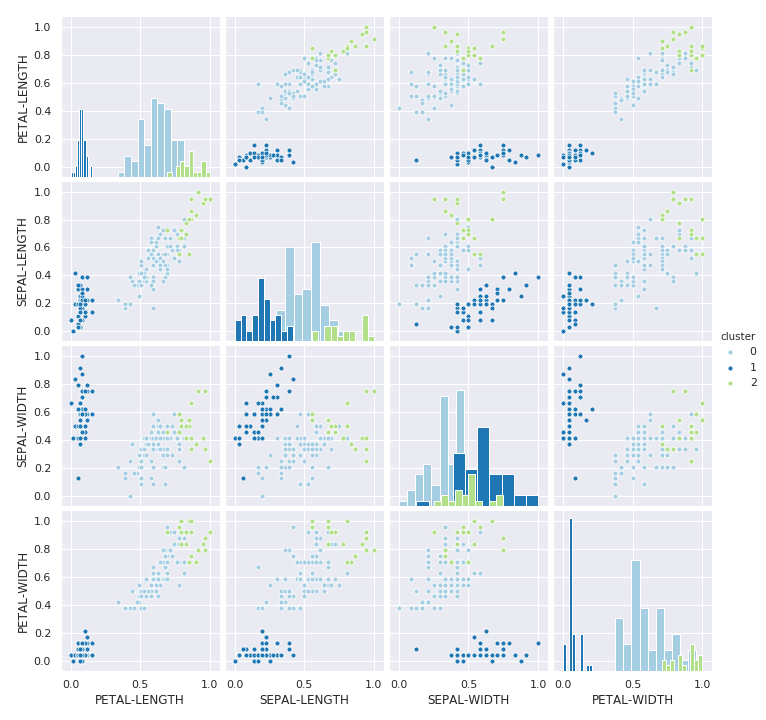
\includegraphics[scale=0.64]{dani/scatmatrixMeanShiftIRIS.png}
\caption{Scatter Matrix para Mean Shift con 3 clústeres.}
\label{smms}
\end{figure}

\clearpage

\begin{figure}[h]
\centering
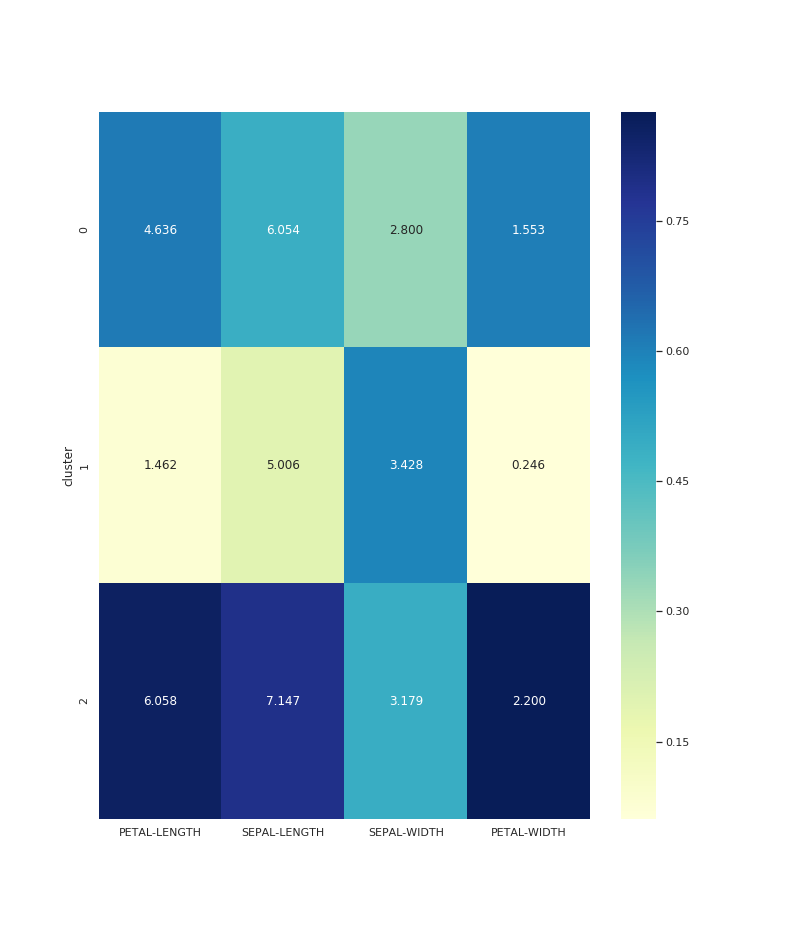
\includegraphics[scale=0.62]{dani/heatmapMeanShiftIRIS.png}
\caption{HeatMap para Mean Shift con 3 clústeres.}
\label{hmms}
\end{figure}

\clearpage

\section{Conclusiones}
El análisis clúster es una metodología de análisis exploratorio de datos. Trata de descubrir cómo algunos objetos se relacionan. Este tipo de análisis depende de la cantidad de ruido en los datos, la existencia de datos anómalos, las variables seleccionadas para el análisis, la medida de proximidad utilizada, las propiedades espaciales de los datos y el método de agrupamiento empleado.

Una ventaja de los métodos jerárquicos sobre los no jerárquicos es que uno no tiene que saber de antemano el número de clústeres (que hemos visto que no es fácil). Además los métodos jerárquicos muchas veces son llamados ``exploratorios'' mientras que los no jerárquicos se denominan ``confirmatorios''. Podemos ver ambos métodos como complementarios. Los métodos jerárquicos no solo dependen de la medida de proximidad utilizada, se ven afectados por el encadenamiento: los objetos tienen a unirse a un clúster existente más que a iniciar uno nuevo.

Un problema importante del \textit{clustering} es la validación de la solución. Para ello deberemos usar criterios internos, externos y métodos de replicación o validación cruzada.

\clearpage
%%%%%%%%%%%%%%%%%%%%%%%%%%%%%%%%%%%%%%%%%%%%%%%%%%%%%%%%%%%%%%%%%%%
%       REFERENCIAS
%%%%%%%%%%%%%%%%%%%%%%%%%%%%%%%%%%%%%%%%%%%%%%%%%%%%%%%%%%%%%%%%%%%
\section{Bibliografía}
\nocite{*}
\bibliographystyle{plain}
\bibliography{referencias.bib}
\end{document}
